%!TEX root = ../report.tex

\begin{document}
    \chapter{Experiments and Results}
    %In this chapter, we will discuss about the experiments conducted for out-of-distribution (OOD) detection on RandLA-Net using uncertainty techniques such as deep ensembles and flipout.
    %These experiments were conducted on Semantic3D dataset as training in-distribution (ID) dataset and two datasets particularly S3DIS and Toronto3D are used as OOD datasets. 
    %The detailed description about datasets can be found in Chapter \textcolor{red}{cite here}, about RandLA-Net in Section \textcolor{red}{cite here}, and about deep ensembles and flipout in Section \textcolor{red}{cite here}
    %The list of experiments conducted to acheive OOD detection are as follows:
    This chapter discusses the experiments conducted for Out-Of-Distribution (OOD) detection on RandLA-Net using quantified uncertainty from Deep Ensembles and Flipout.
    In a detailed discussion about RandLA-Net, Deep Ensembles and Flipout can be found in Chapter~[\$]. In this chapter, we first discuss the training results of RandLA-Net using deep ensembles and flipout on Semantic3D as an In-Distribution (ID) dataset.
    Furthermore, we compare the Maximum Softmax Probability (MSP) as in \cite{hendrycks2016baseline_MSP} and entropy values for the proposed OOD benchmark datasets Semantic3D vs S3DIS and Semantic3D vs Semantic3D w/o colour.
    Finally, we visualize and evaluate the performance of OOD detection using the AUROC score.

%%%%%%%%%%%%%%%%%%%%%%%%%%%%%%%%%%%%%%%%%%%%%%%%%%%%%%%%%%%%%%%%%%%%%%%%%%%%%%%
    %%%%%% Deep ensmebles performance %%%%%%
    \section{Deep Ensembles-Semantic3D}
    \label{sec:deepensemble_train}
    In this experiment, we trained 20 models of RandLA-Net over the Semantic3D dataset using random initializations with the experimental setup described in Section~[\$].
    The predictions from these 20 individual models are then averaged to compute the final predictions.
    The evaluation results of the Deep Ensembles are described in Table~\ref{tab:ensemble_eval} using meanIoU, per-class IoU and accuracy.
    The predictions from the Deep Ensembles are depicted in Figure~\ref{fig:deepensemble_vis_sem3d} and Figure~\ref{fig:deepensemble_improv}.
    \begin{table}[h!]
        \resizebox{\textwidth}{!}{%
        \begin{tabular}{c|c|cccccccc|c}
        %\textbf{\#Ensembles} & \textbf{MeanIOU} & \textbf{Accuracy} & \textbf{Manmadeterrain} & \textbf{Naturalterrain} & \textbf{Highvegetation} & \textbf{Lowvegetation} & \textbf{Buildings} & \textbf{Hardscapes} & \textbf{Scanningartifacts} & \textbf{Cars} \\ \hline
        & & \multicolumn{7}{c}{\textbf{IoU per class}} & \\ \hline
        \textbf{Ensemble size} & \textbf{meanIoU} & \textbf{C1} & \textbf{C2} & \textbf{C3} & \textbf{C4} & \textbf{C5} & \textbf{C6} & \textbf{C7} & \textbf{C8} & \textbf{Accuracy} \\ \hline
        1& 68.19& 94.55& 81.19& 84.67& 29.43& 81.37& 18.85& 64.74& 90.74& 88.78 \\
        5& 69.51& 94.73& 81.92& 84.42& 28.05& \textbf{86.41}& 28.50& 61.03& 91.03& 90.04 \\
        10& 69.97& 95.25& 83.73& 86.63& 30.36& 84.13& 18.60& \textbf{66.01}& 92.61& 89.94 \\
        15& 70.32& 95.27& 83.54& \textbf{88.22}& \textbf{32.19}& 84.82& 26.17& 61.67& 90.75& \textbf{90.57} \\
        20& \textbf{70.80}& \textbf{95.55}& \textbf{84.11}& 86.65& 29.60& 85.41& \textbf{29.58}& 62.47& \textbf{93.06}& 90.56 \\
        \end{tabular}%
        }
        \caption{Illustration of performance of RandLA-Net on Semantic3D over number of ensembles. meanIOU and IOU per-class and overall accuracy are represented here.
        C1 to C8 are the classes of Semantic3D which are Manmadeterrain, Naturalterrain, Highvegetation, Lowvegetation, Buildings, Hardscapes, Scanningartifacts, and Cars.}
        \label{tab:ensemble_eval}
    \end{table} 

    \begin{figure*}[h!]
        \begin{tabular}{ccc}
            RGB & Ground Truth & Prediction \\
            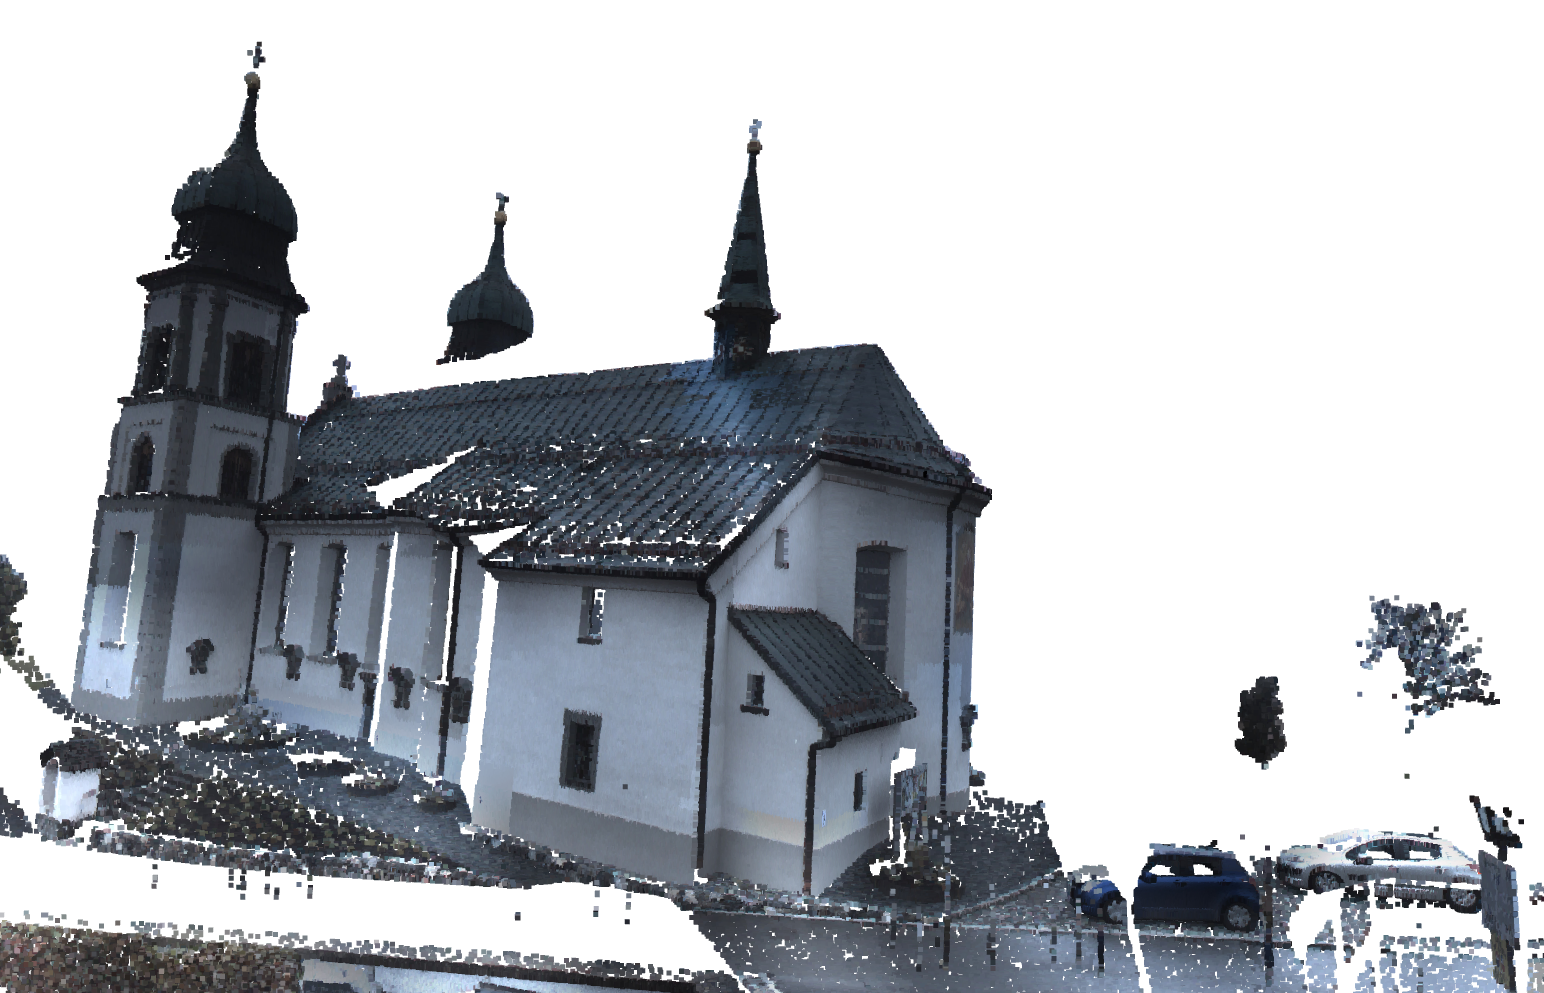
\includegraphics[width=0.33\textwidth, height=0.18\textheight]{images/seg_output/sem3d_seg_output/1_RGB.png} &
            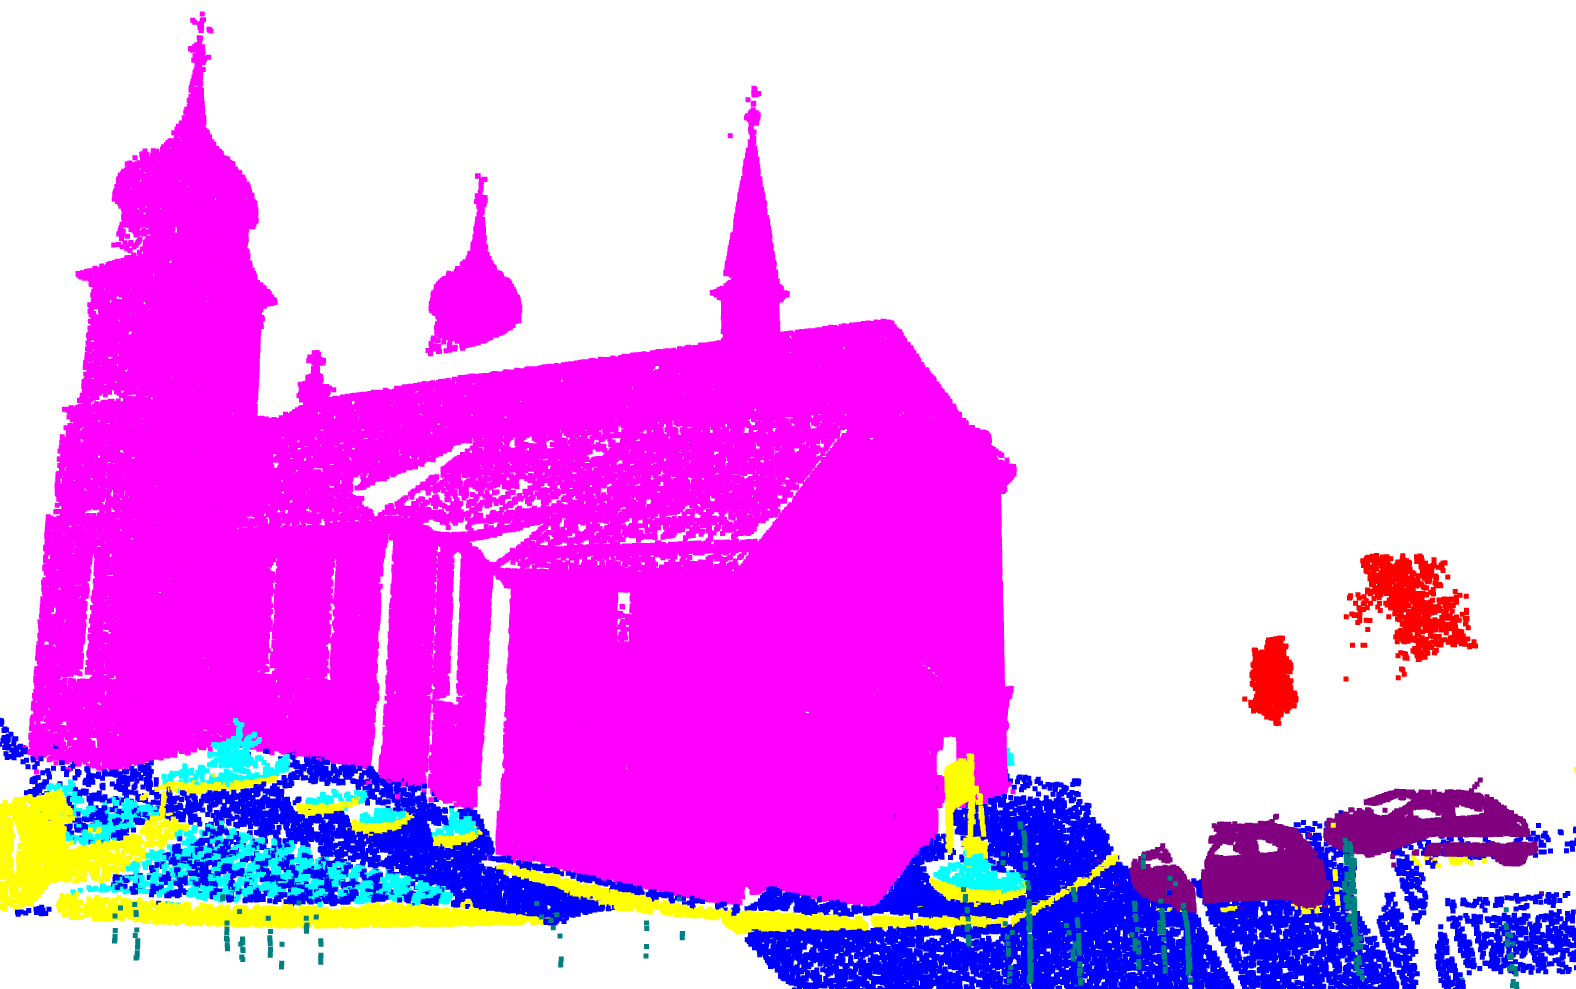
\includegraphics[width=0.33\textwidth, height=0.18\textheight]{images/seg_output/sem3d_seg_output/1_GT.png}& 
            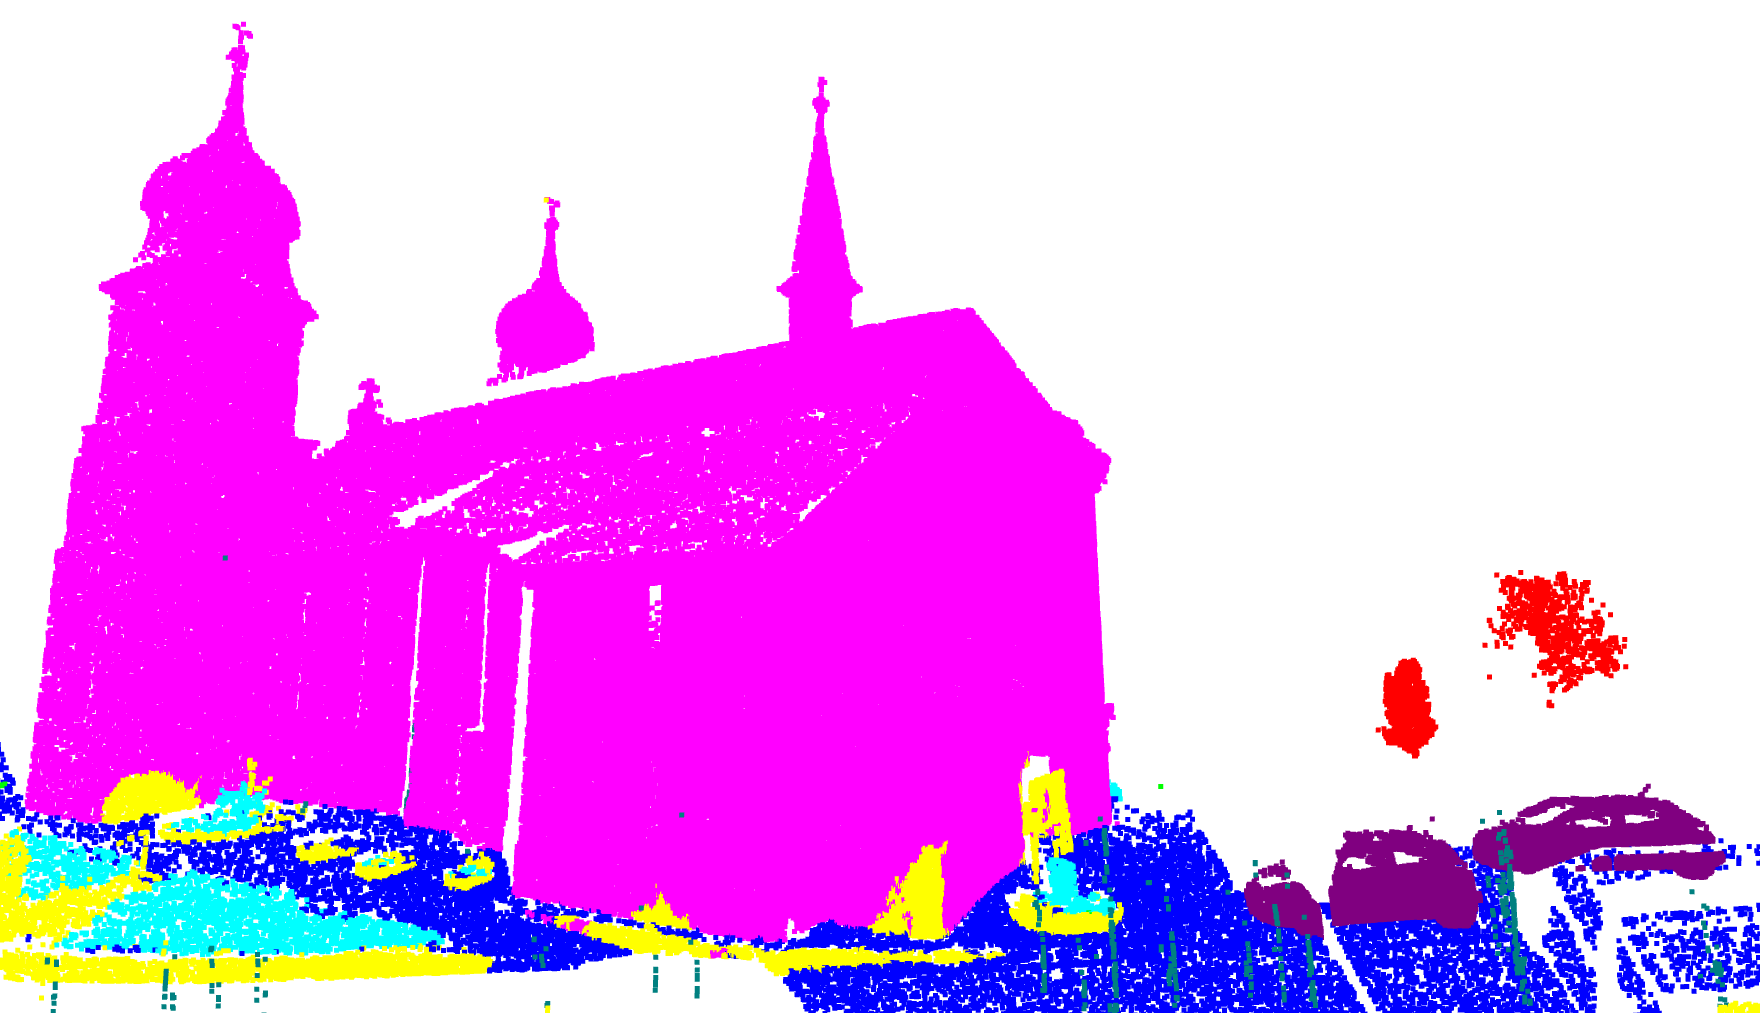
\includegraphics[width=0.33\textwidth, height=0.18\textheight]{images/seg_output/sem3d_seg_output/1_Pred.png}\\

            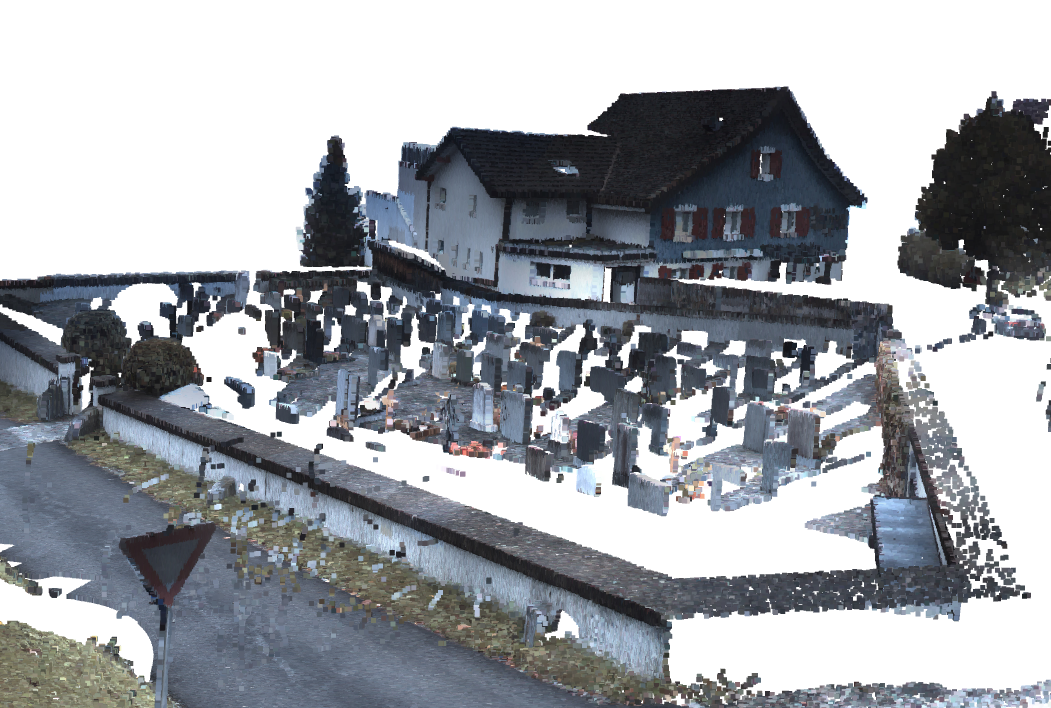
\includegraphics[width=0.33\textwidth, height=0.18\textheight]{images/seg_output/sem3d_seg_output/2_RGB.png} &
            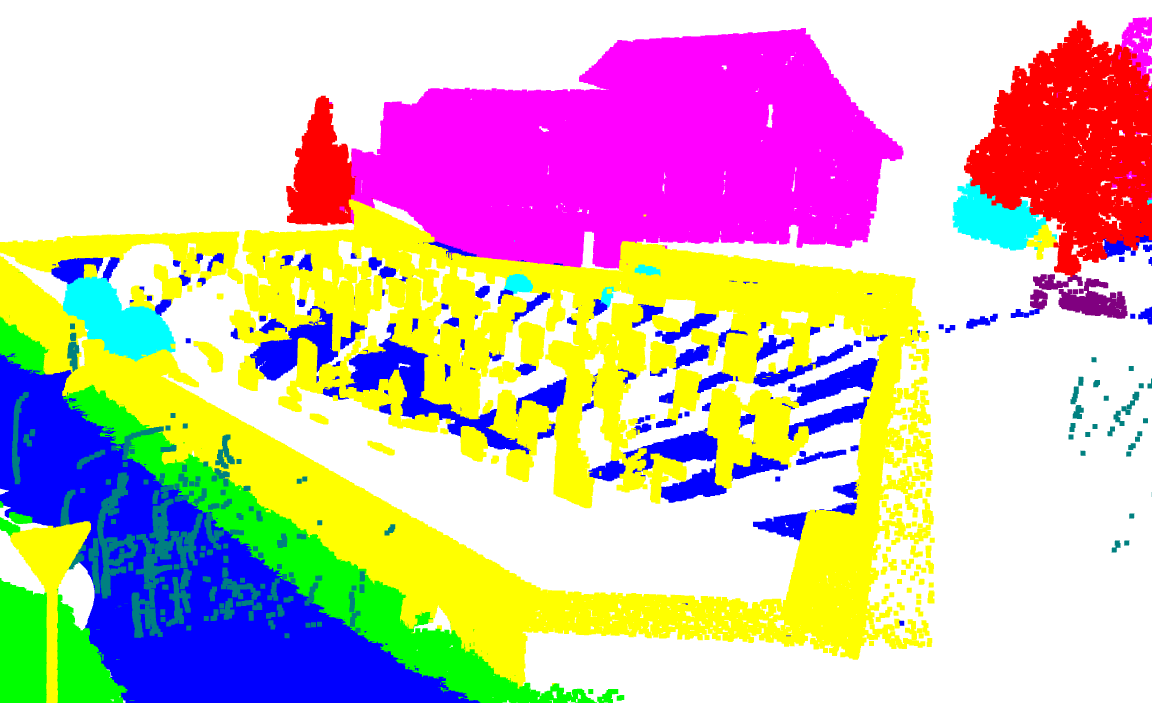
\includegraphics[width=0.33\textwidth, height=0.18\textheight]{images/seg_output/sem3d_seg_output/2_GT.png}& 
            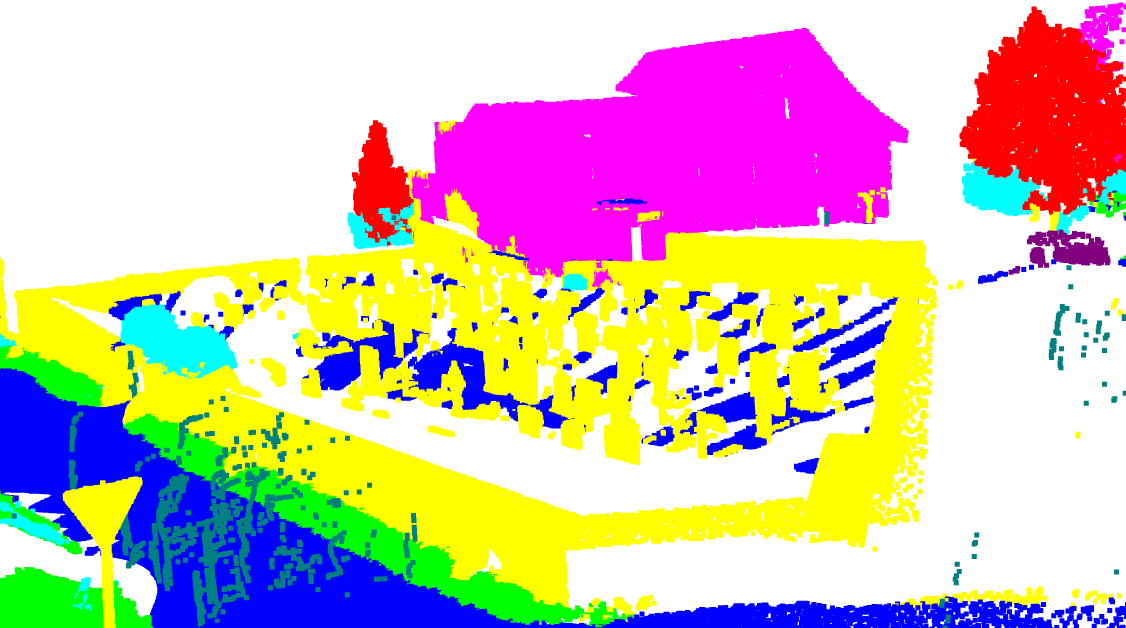
\includegraphics[width=0.33\textwidth, height=0.18\textheight]{images/seg_output/sem3d_seg_output/2_Pred.png}\\

            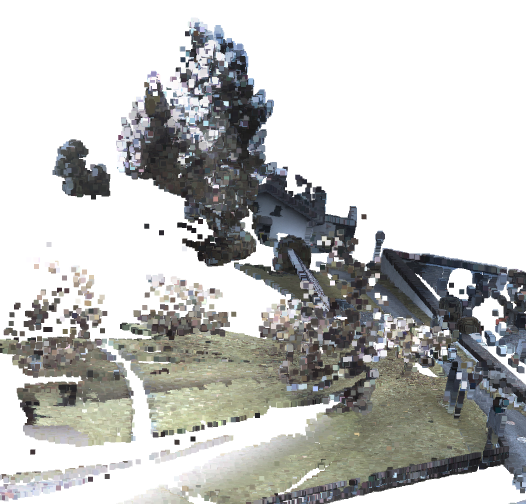
\includegraphics[width=0.33\textwidth, height=0.18\textheight]{images/seg_output/sem3d_seg_output/3_RGB.png} &
            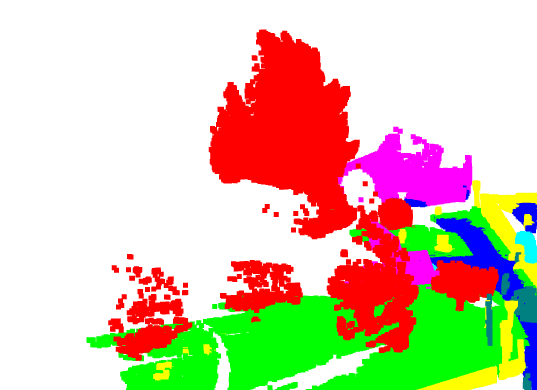
\includegraphics[width=0.33\textwidth, height=0.18\textheight]{images/seg_output/sem3d_seg_output/3_GT.png}& 
            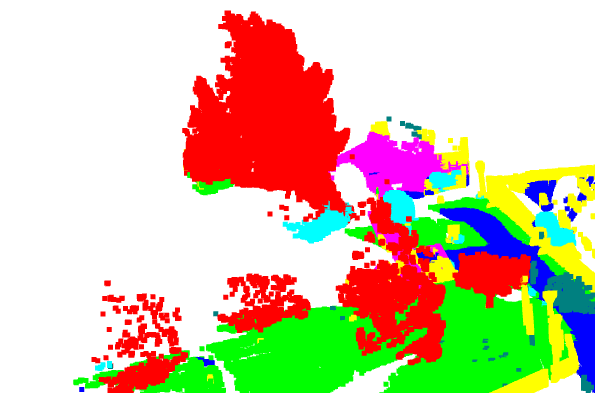
\includegraphics[width=0.33\textwidth, height=0.18\textheight]{images/seg_output/sem3d_seg_output/3_Pred.png}\\
        \end{tabular}
        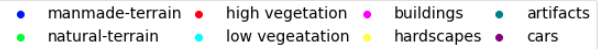
\includegraphics[scale=0.65]{images/legend.png}
        \caption{Output predictions of the RandLA-Net over the Semantic3D dataset (13 ensemble size) \textcolor{red}{Legend spelling mistake}.}
        \label{fig:deepensemble_vis_sem3d}
    \end{figure*}

    % %%%%%% Segmentation output here %%%%%%
    
    % %%%%%% Ensembles output here %%%%%%
    \begin{figure*}[h!]
        \begin{tabular}{cccc}
            1 & 5 & 10 \\
            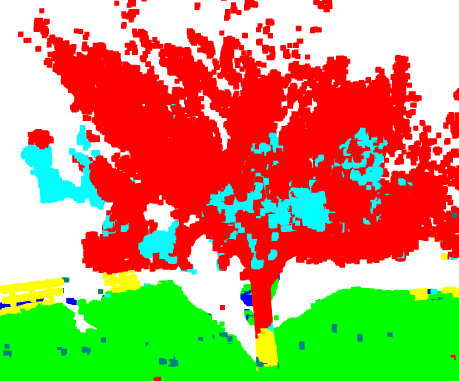
\includegraphics[width=0.30\textwidth, height=0.15\textheight]{images/seg_output/deep_ensembles/1_1.png} &
            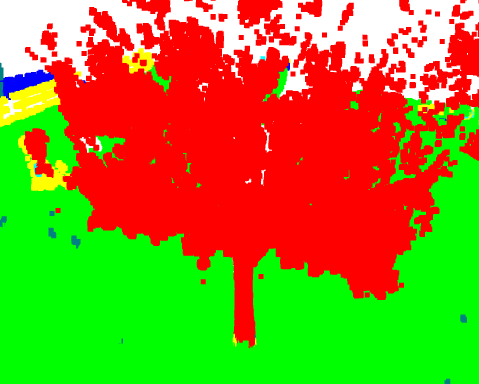
\includegraphics[width=0.30\textwidth, height=0.15\textheight]{images/seg_output/deep_ensembles/1_5.png}& 
            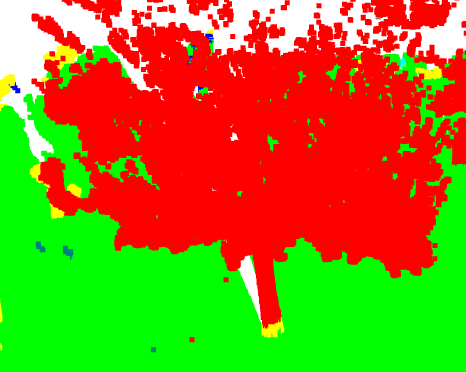
\includegraphics[width=0.30\textwidth, height=0.15\textheight]{images/seg_output/deep_ensembles/1_10.png}\\

            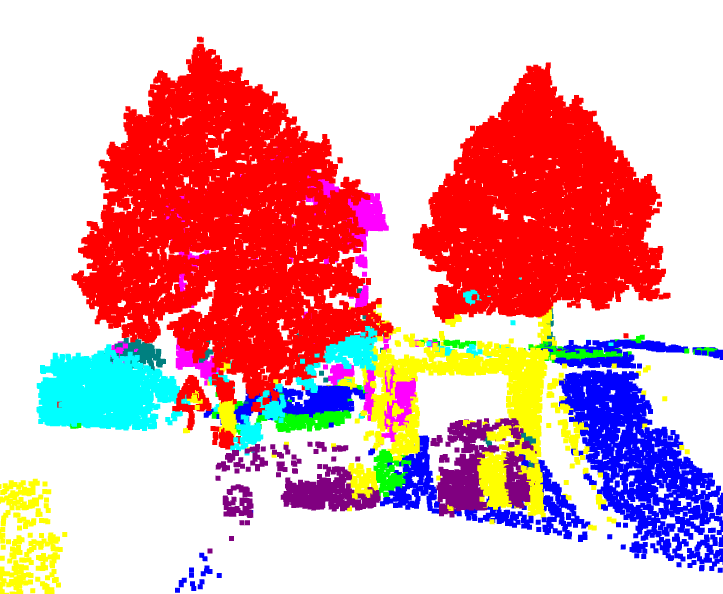
\includegraphics[width=0.30\textwidth, height=0.15\textheight]{images/seg_output/deep_ensembles/2_1.png} &
            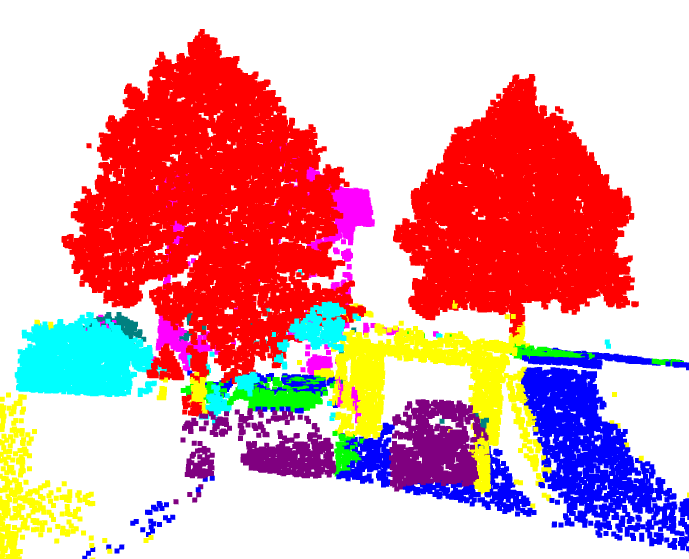
\includegraphics[width=0.30\textwidth, height=0.15\textheight]{images/seg_output/deep_ensembles/2_5.png}& 
            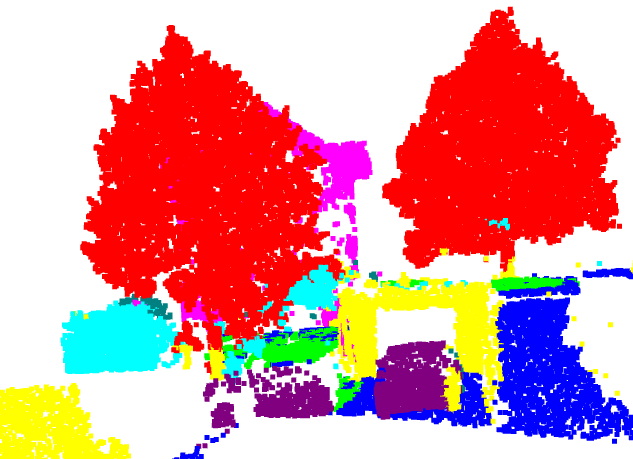
\includegraphics[width=0.30\textwidth, height=0.15\textheight]{images/seg_output/deep_ensembles/2_10.png}\\
        \end{tabular}
        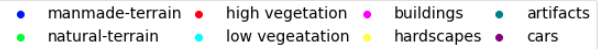
\includegraphics[scale=0.65]{images/legend.png}
        \caption{Deep ensembles performance on RandLA-Net over the Semantic3D dataset.}
        \label{fig:deepensemble_improv}
    \end{figure*}

    From the Table~\ref{tab:ensemble_eval}, we infer that the Deep Ensembles improve the model's overall performance in terms of meanIoU and Accuracy.
    With an ensemble size of 10, we observe a 2\% increment in meanIoU.
    An increase in ensemble size also results in an improvement in per-class IoU performance.
    Figure~\ref{fig:deepensemble_improv} depicts the improvement in model classifications visually with the increase in ensemble size.
    From Figure~\ref{fig:deepensemble_vis_sem3d}, we also observe the misclassifications along the edges of the church, trees and ground.
    The possible explanation for these misclassifications is ambiguity in the feature vector of RandLA-Net. For example, a feature vector for the point along the lower edge of the church contains the part of ground points as the feature vector.
%%%%%%%%%%%%%%%%%%%%%%%%%%%%%%%%%%%%%%%%%%%%%%%%%%%%%%%%%%%%%%%%%%%%%%%%%%%%%%%
    \section{Flipout-Semantic3D}
    In this experiment, we trained a Flipout version of RandLA-Net as described in Section~[\$] over the Semantic3D dataset.
    Like Deep Ensembles, we performed 20 forward passes over the Flipout versioned RandLA-Net and averaged the predictions to obtain final predictions.
    Table~\ref{tab:flipout_eval} describes the performance of Flipout versioned RandLA-Net using meanIoU, per-class IoU and Accuracy.
    Figure~\ref{fig:flipout_vis_sem3d} depicts the predictions of the Flipout versioned RandLA-Net visually.
    \begin{table}[h!]
        \resizebox{\textwidth}{!}{%
        \begin{tabular}{c|c|cccccccc|c}
        %\textbf{\#Ensembles} & \textbf{MeanIOU} & \textbf{Accuracy} & \textbf{Manmadeterrain} & \textbf{Naturalterrain} & \textbf{Highvegetation} & \textbf{Lowvegetation} & \textbf{Buildings} & \textbf{Hardscapes} & \textbf{Scanningartifacts} & \textbf{Cars} \\ \hline
        & & \multicolumn{7}{c}{\textbf{IoU per class}} & \\ \hline
        \textbf{\#Passes} & \textbf{MeanIoU} & \textbf{C1} & \textbf{C2} & \textbf{C3} & \textbf{C4} & \textbf{C5} & \textbf{C6} & \textbf{C7} & \textbf{C8} & \textbf{Accuracy} \\ \hline
        1& 69.95  & 94.24&80.09&86.16&22.48&88.70&39.41&57.42&91.12&90.71\\
        5& 69.83  & 94.38&80.21&84.10&23.32&87.80&39.68&57.75&91.43&90.43\\
        10& 69.84 & 94.38&80.16&83.90&23.46&87.73&39.75&57.83&91.47&90.40\\
        15& 69.86 & 94.38&80.17&83.80&23.48&87.73&39.82&57.96&91.57&90.40\\
        20& 69.87 & 94.38&80.18&83.80&23.57&87.72&39.84&57.92&91.57&90.40\\
        \end{tabular}%
        }
        \caption{Illustration of performance of Flipout versioned RandLA-Net on Semantic3D. meanIOU and IOU per-class and overall accuracy are represented here.
        C1 to C8 are the classes of Semantic3D which are Manmadeterrain, Naturalterrain, Highvegetation, Lowvegetation, Buildings, Hardscapes, Scanningartifacts, and Cars.}
        \label{tab:flipout_eval}
    \end{table}
    \begin{figure*}[h!]
        \begin{tabular}{ccc}
            RGB & Ground Truth & Prediction \\
            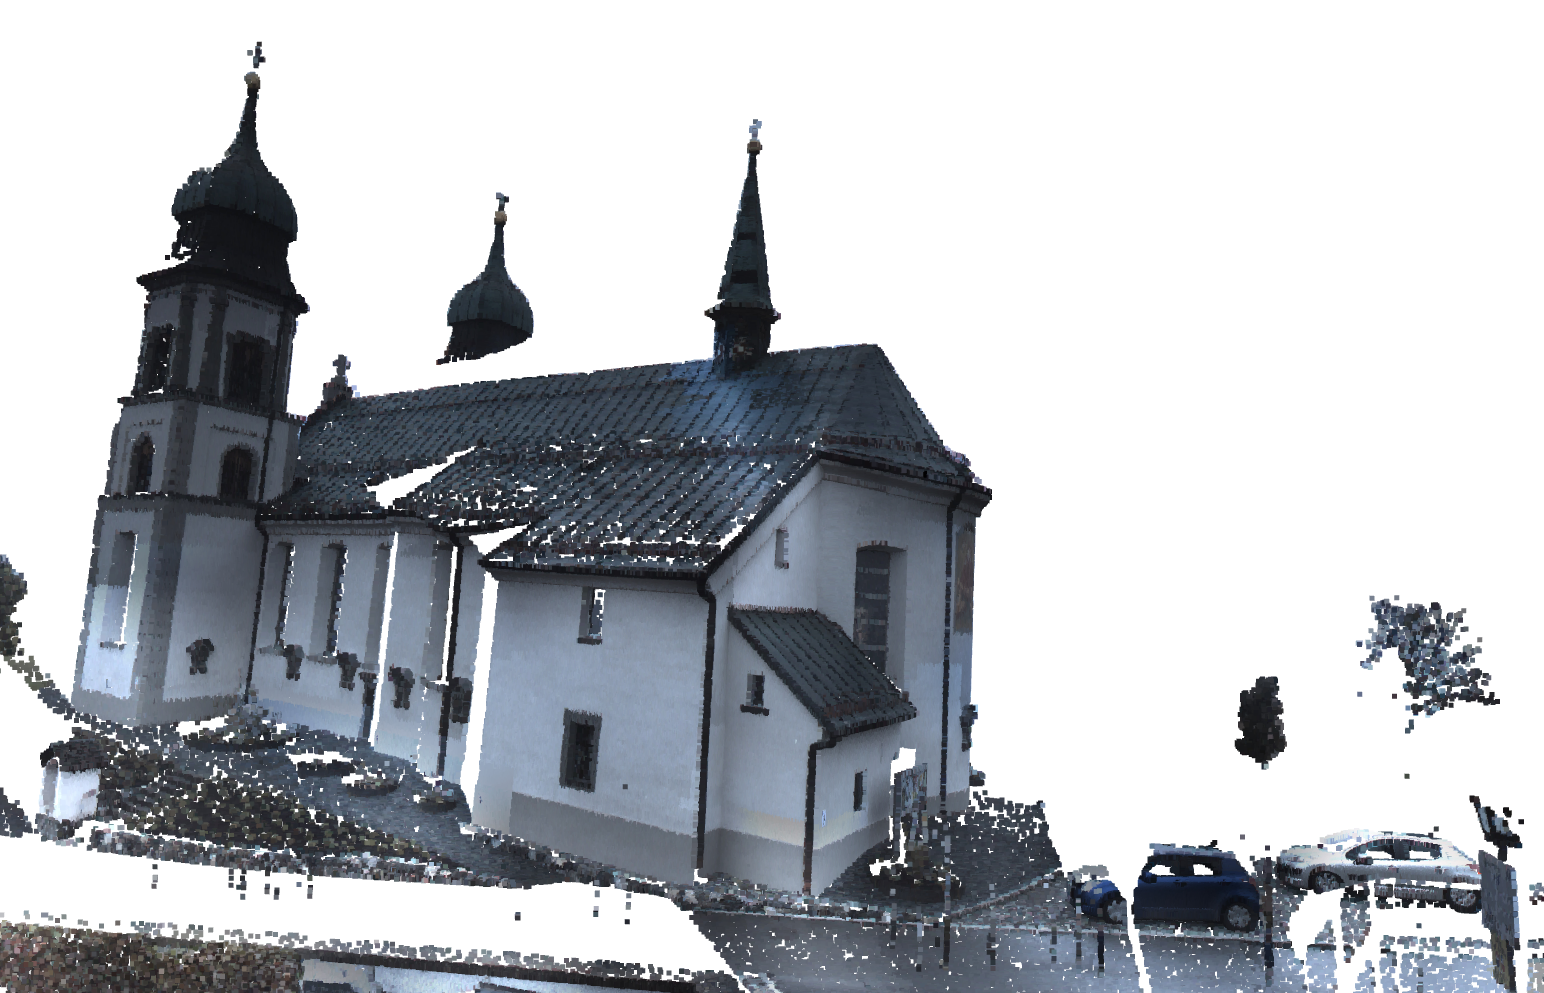
\includegraphics[width=0.33\textwidth, height=0.18\textheight]{images/seg_output/sem3d_seg_output/1_RGB.png} &
            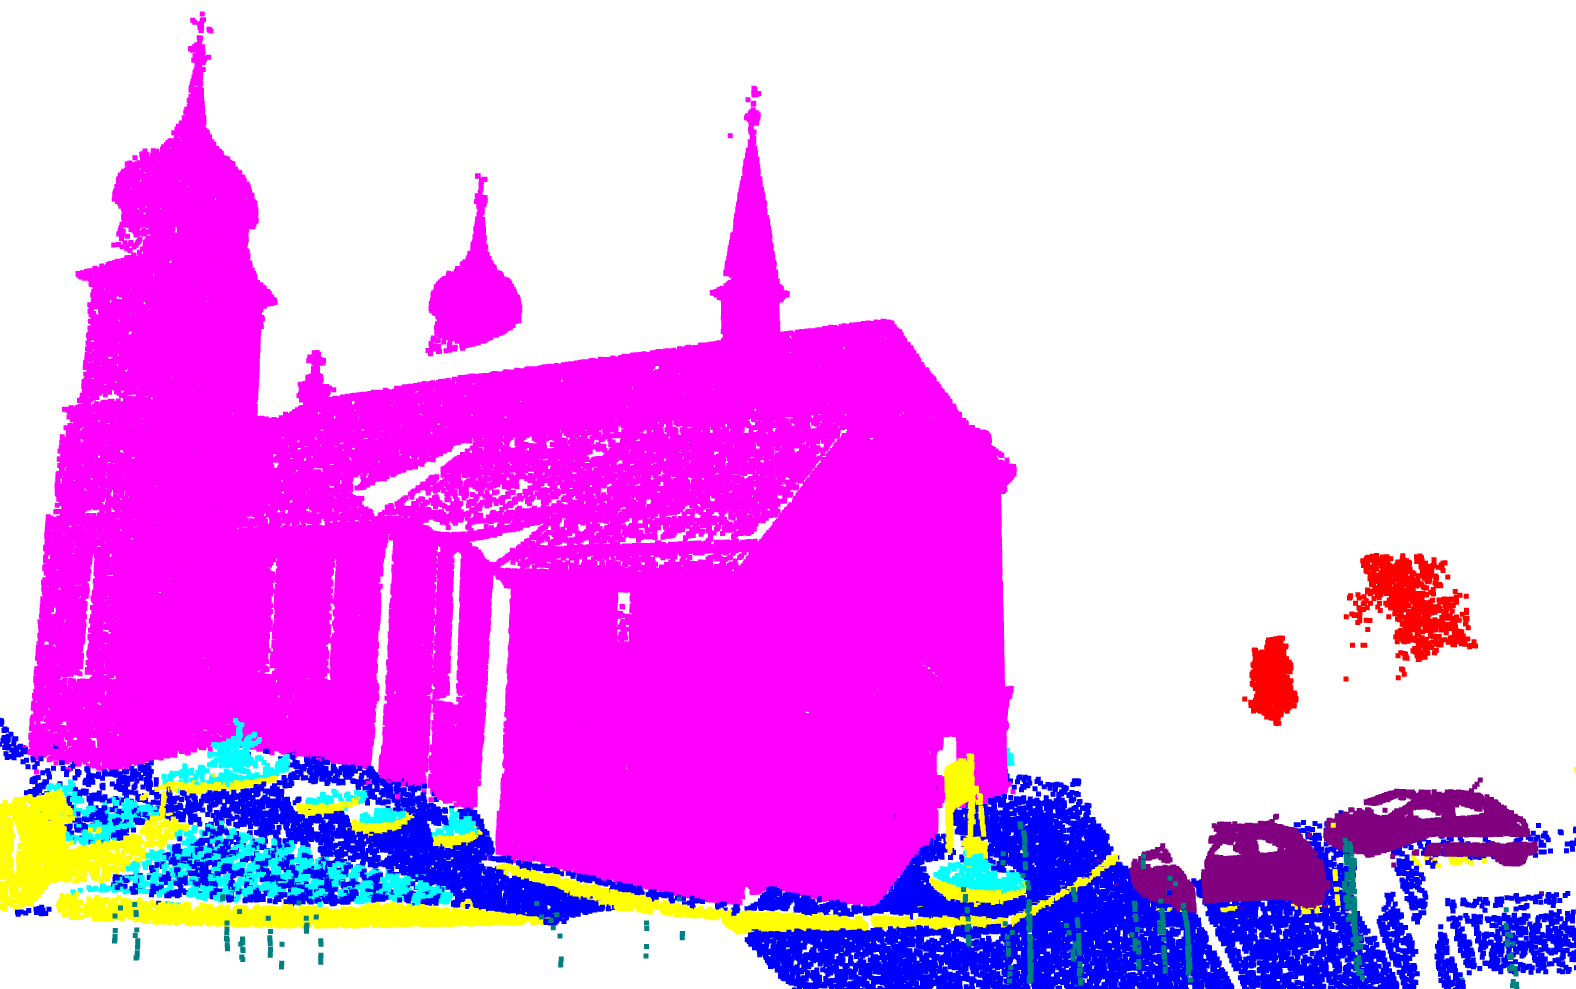
\includegraphics[width=0.33\textwidth, height=0.18\textheight]{images/seg_output/sem3d_seg_output/1_GT.png}& 
            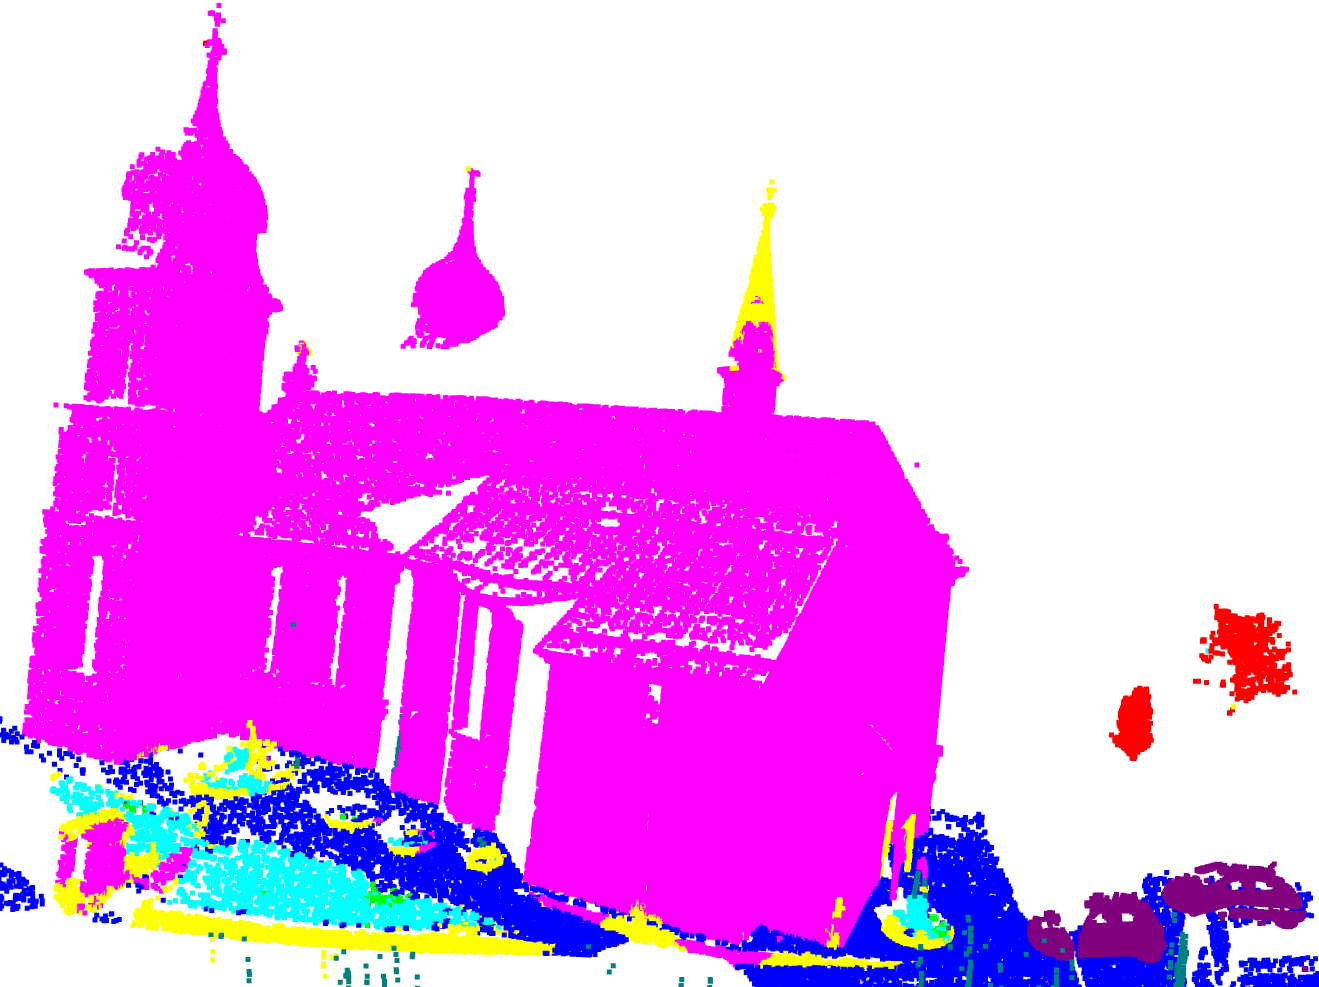
\includegraphics[width=0.33\textwidth, height=0.18\textheight]{images/seg_output/flipout/sem3d_1.png}\\

            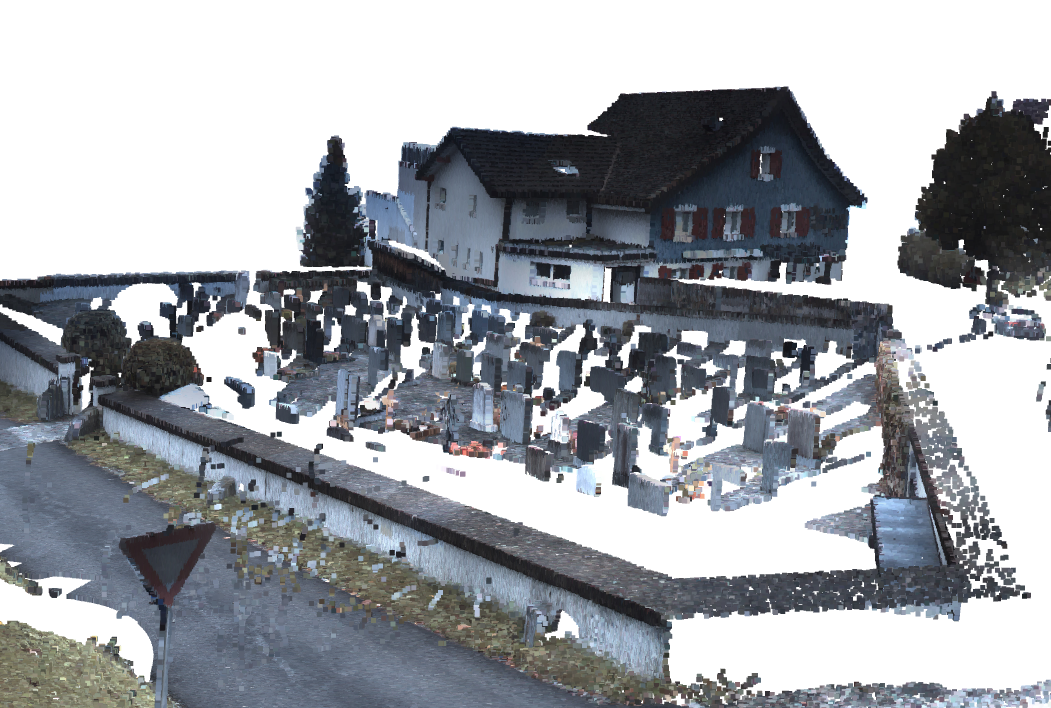
\includegraphics[width=0.33\textwidth, height=0.18\textheight]{images/seg_output/sem3d_seg_output/2_RGB.png} &
            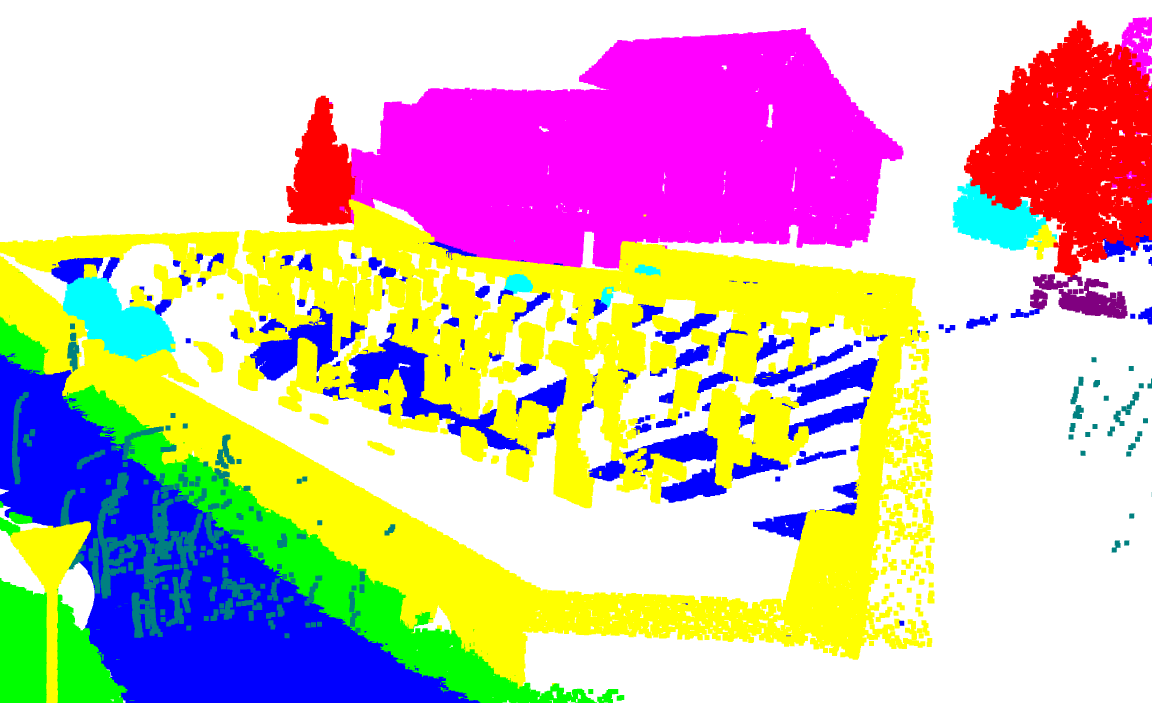
\includegraphics[width=0.33\textwidth, height=0.18\textheight]{images/seg_output/sem3d_seg_output/2_GT.png}& 
            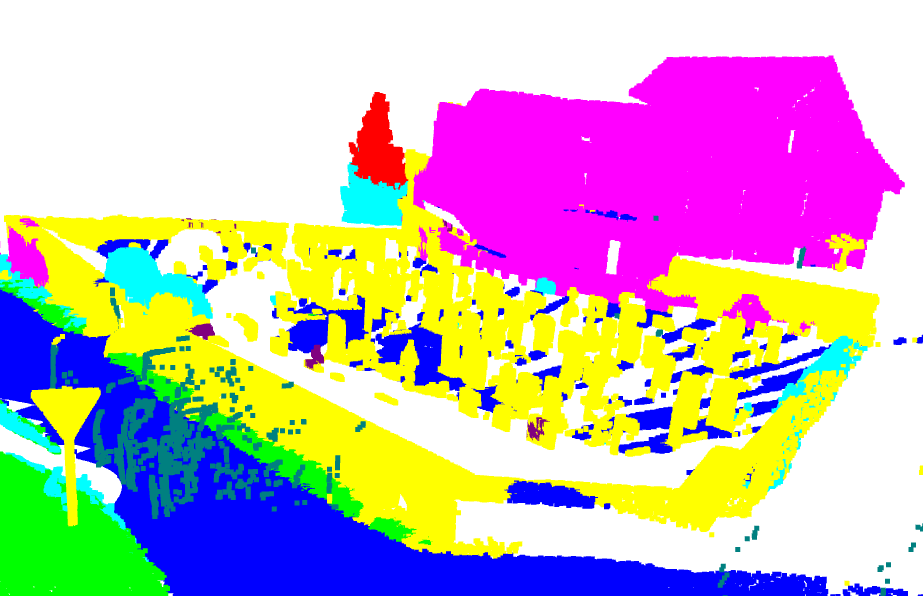
\includegraphics[width=0.33\textwidth, height=0.18\textheight]{images/seg_output/flipout/sem3d_2.png}\\

            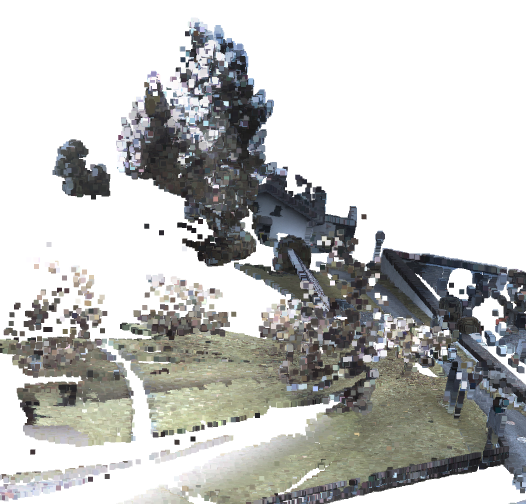
\includegraphics[width=0.33\textwidth, height=0.18\textheight]{images/seg_output/sem3d_seg_output/3_RGB.png} &
            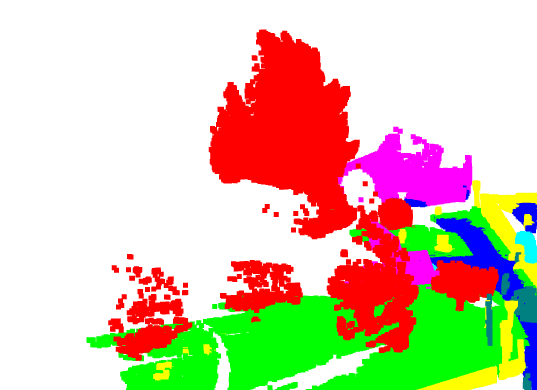
\includegraphics[width=0.33\textwidth, height=0.18\textheight]{images/seg_output/sem3d_seg_output/3_GT.png}& 
            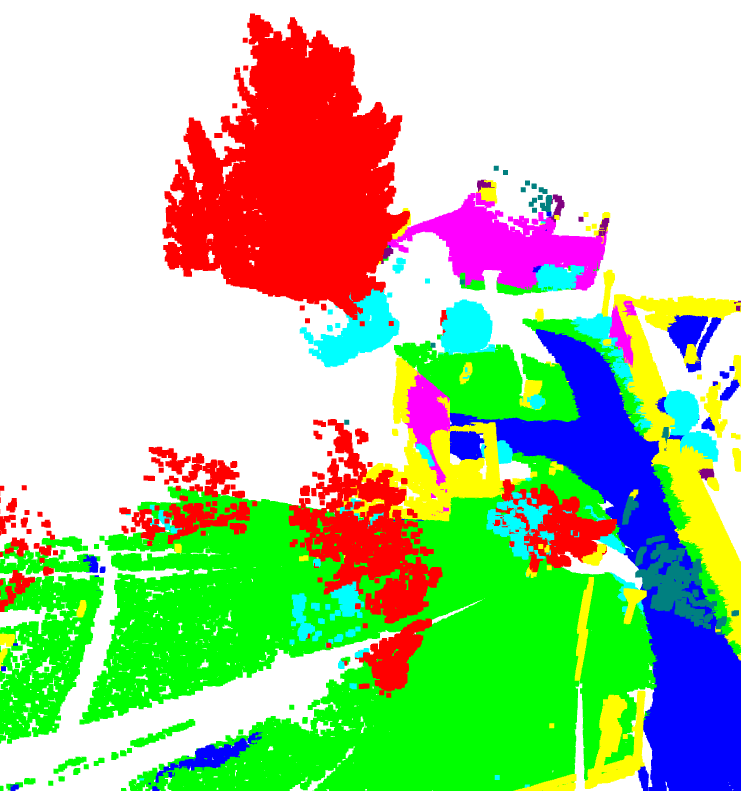
\includegraphics[width=0.33\textwidth, height=0.18\textheight]{images/seg_output/flipout/sem3d_3.png}\\
        \end{tabular}
        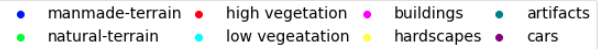
\includegraphics[scale=0.65]{images/legend.png}
        \caption{Output predictions of the RandLA-Net over the Semantic3D dataset (10 forward passes) \textcolor{red}{Legend spelling mistake}.}
        \label{fig:flipout_vis_sem3d}
    \end{figure*}   

    From Table~\ref{tab:flipout_eval}, we infer that the Flipout versioned RandLA-Net has a similar performance to the original RandLA-Net model proposed in \cite{Hu_2020_CVPR_Randla} and also Deep Ensembles with ensemble size one .
    We also observe a significant improvement in the Hardscapes class represented as C6 in Table~\ref{tab:flipout_eval}.
    There is a decrement in performance of classes Lowvegetation represented as C4 and Scanningartifacts represented as C7 in Table~\ref{tab:flipout_eval}, keeping the overall meanIoU same.
    % \textcolor{red}{Add the images of flipout performance here same as figures in deep ensembles}
    
%%%%%%%%%%%%%%%%%%%%%%%%%%%%%%%%%%%%%%%%%%%%%%%%%%%%%%%%%%%%%%%%%%%%%%%%%%%%%%%
    \section{OOD benchmark - Semantic3D vs S3DIS}
    In the previous section, we studied the performance of the Deep Ensembles and Flipout over the Semantic3D (In-Distribution) dataset.
    In this section, we study the predictions of the RandLA-Net model on the S3DIS (Out-Of-Distribution) dataset using Deep Ensembles and Flipout.
    We also compare the distribution of Maximum Softmax Probability (MSP) and entropy scores for Semantic3D and S3DIS datasets.

    Figure~\ref{fig:de_s3dis_vis} depicts the predictions of the RandLA-Net model and Flipout versioned RandLA-Net.
    We observe that most objects, such as ceilings and bookshelves, are labelled as buildings when using Deep Ensembles.
    We also observe that most point clouds are labelled as hardscapes class when using Flipout versioned RandLA-Net.
    The classifications on S3DIS datasets are in triangles because of the property of the scanner.
    As discussed in Section~[\$], data collected from the Matterport scanner is represented as triangular mesh, and then a point cloud is extracted from this mesh.

    \begin{figure*}[h!]
        \centering
        \begin{tabular}{ccc}
            RGB & Deep Ensembles & Flipout \\
            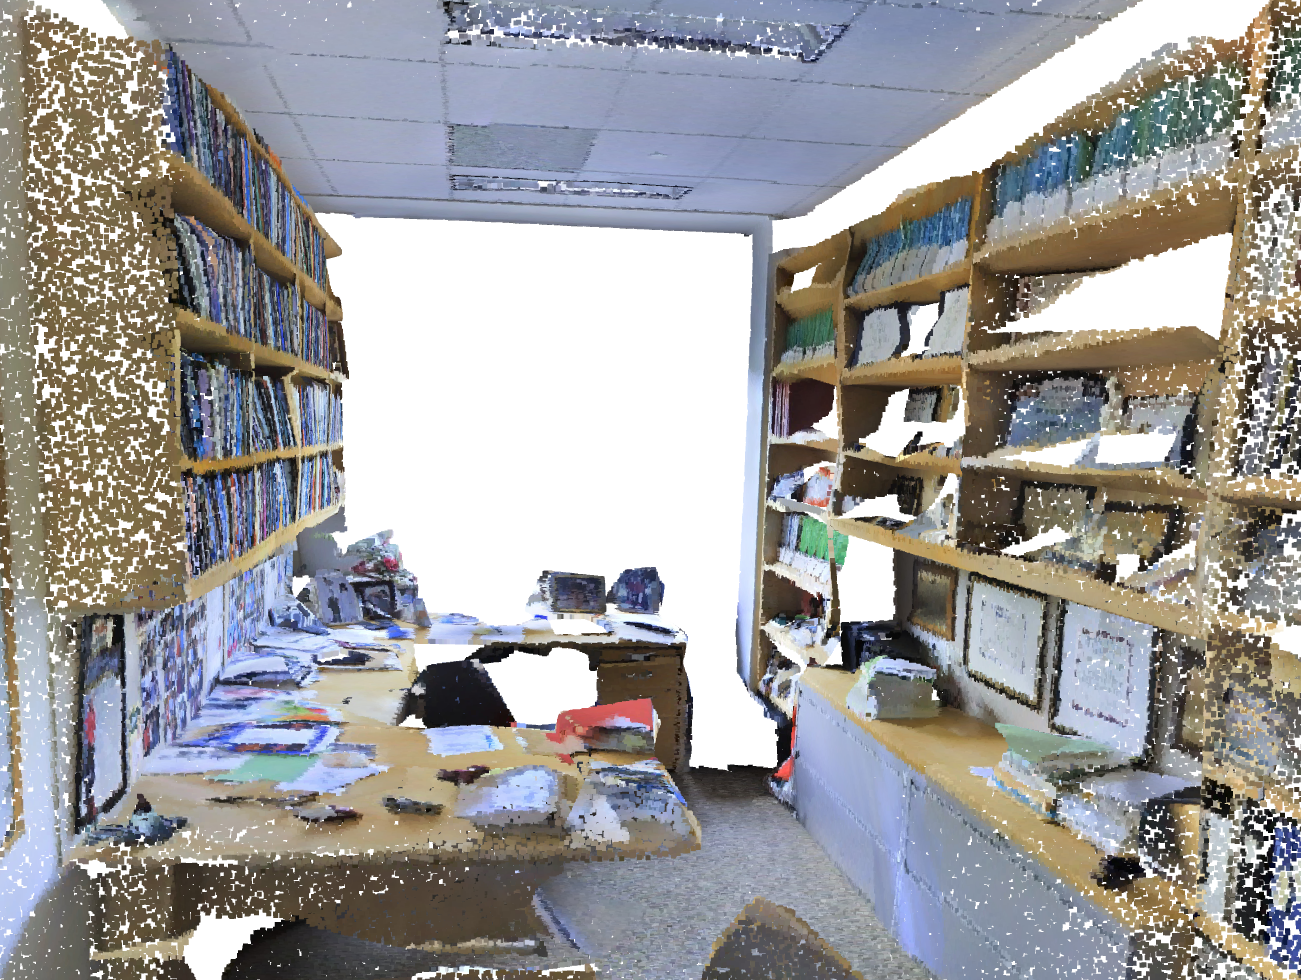
\includegraphics[width=0.33\textwidth, height=0.18\textheight]{images/seg_output/s3dis_DE/S3DIS_1_RGB.png} &
            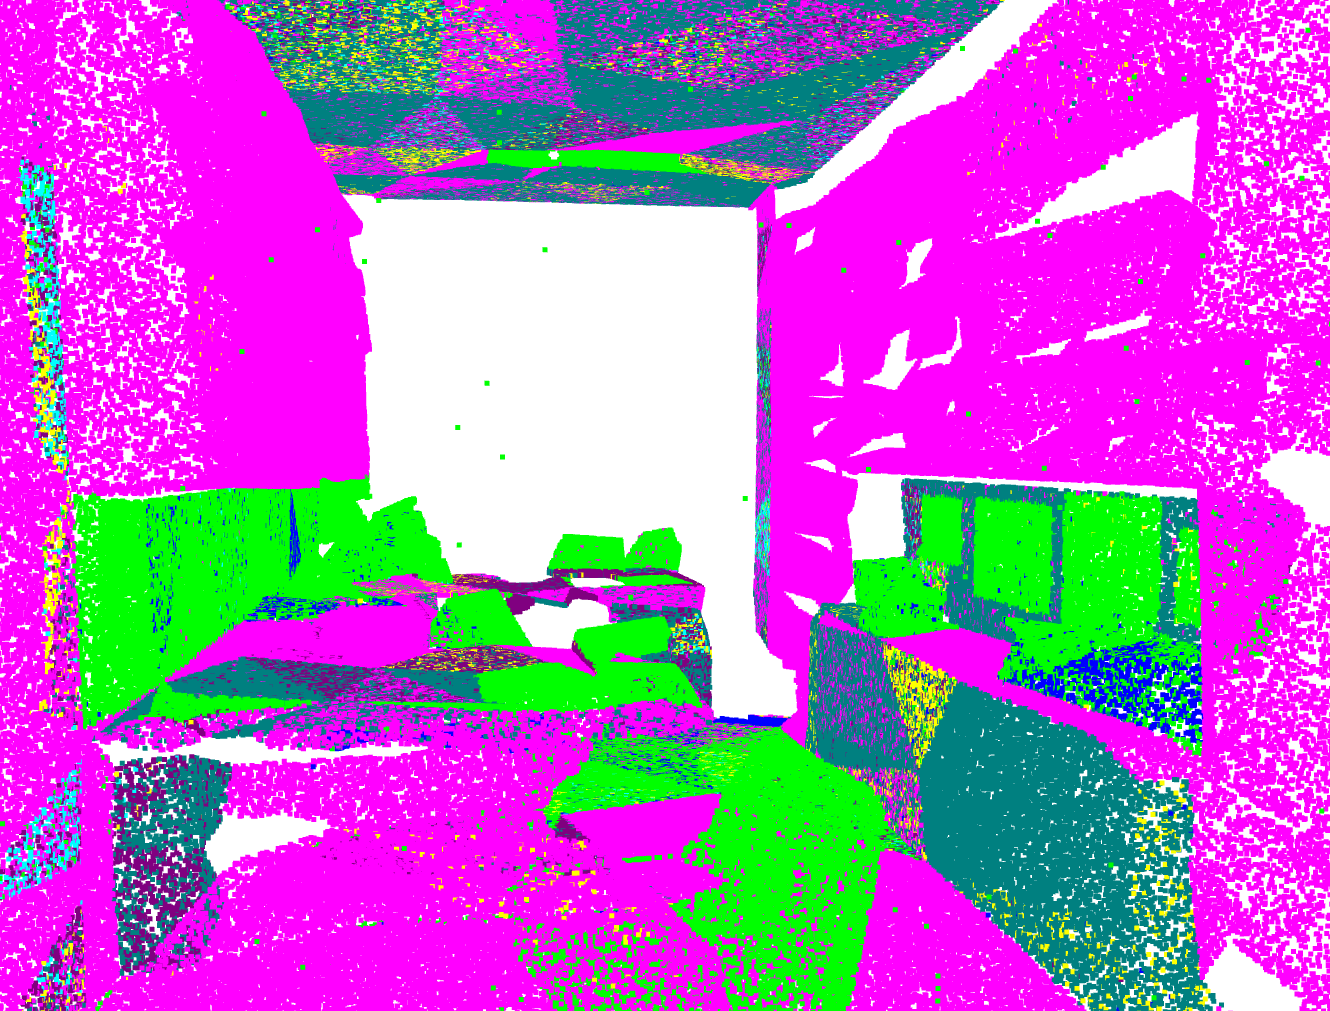
\includegraphics[width=0.33\textwidth, height=0.18\textheight]{images/seg_output/s3dis_DE/S3DIS_1_Pred.png} &
            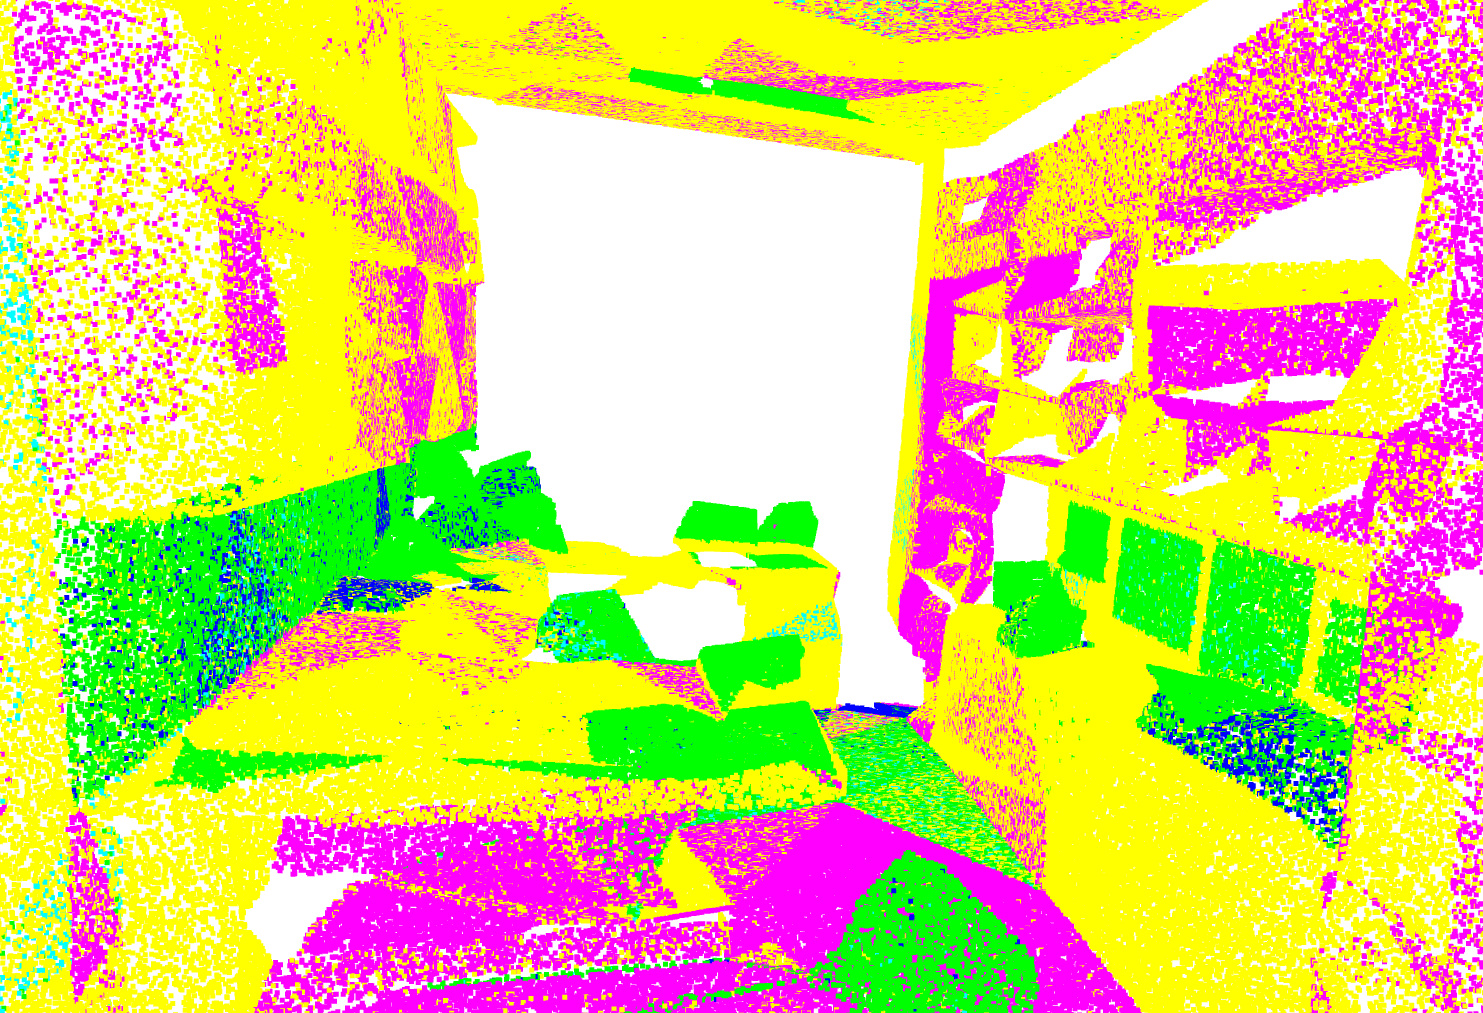
\includegraphics[width=0.33\textwidth, height=0.18\textheight]{images/seg_output/s3dis_DE/office_3.png} \\

            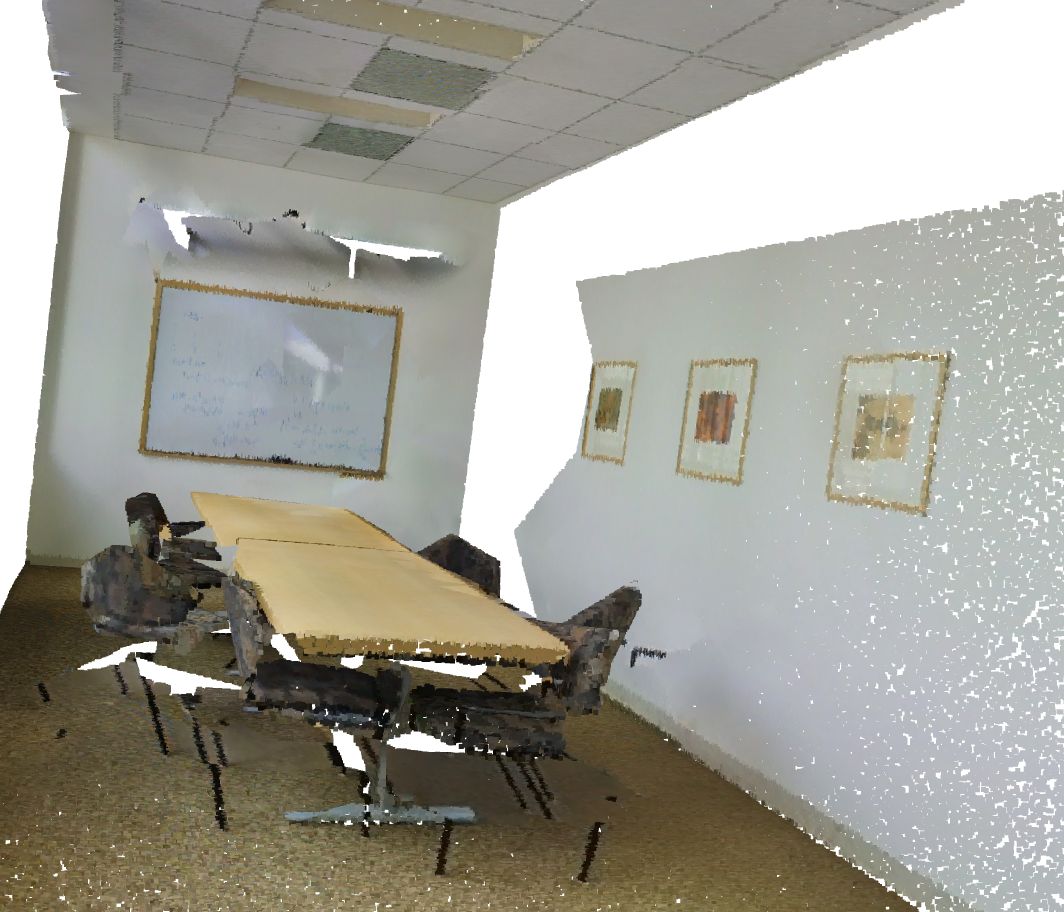
\includegraphics[width=0.33\textwidth, height=0.18\textheight]{images/seg_output/s3dis_DE/S3DIS_2_RGB.png} &
            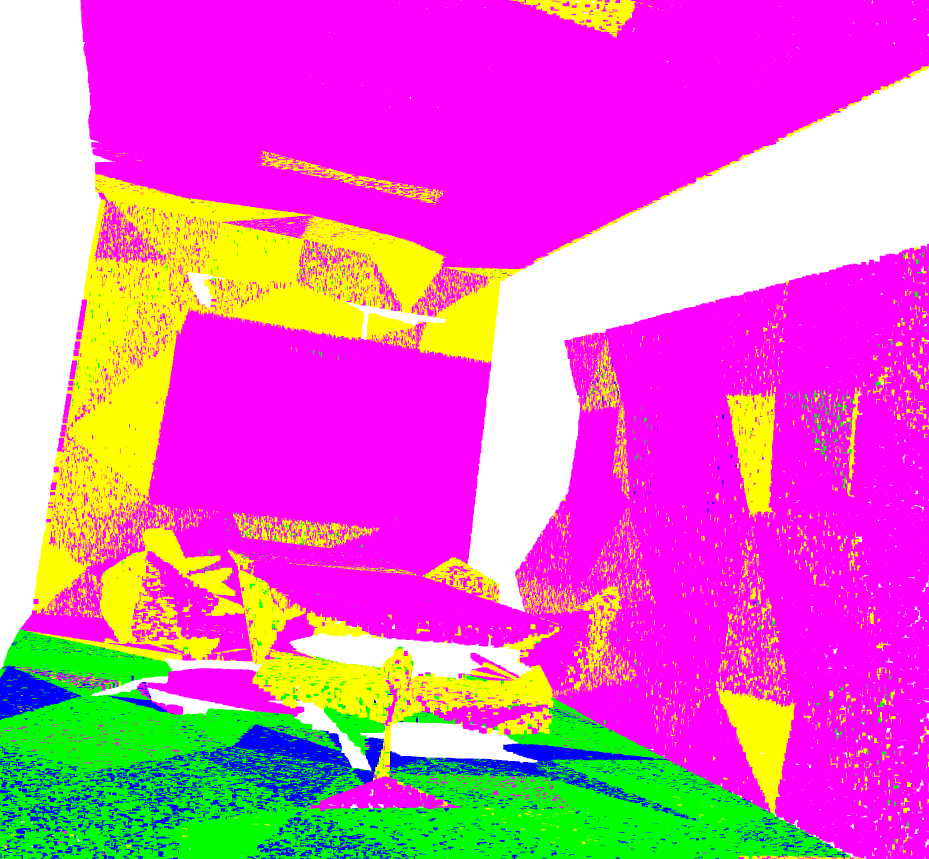
\includegraphics[width=0.33\textwidth, height=0.18\textheight]{images/seg_output/s3dis_DE/S3DIS_2_Pred.png}&
            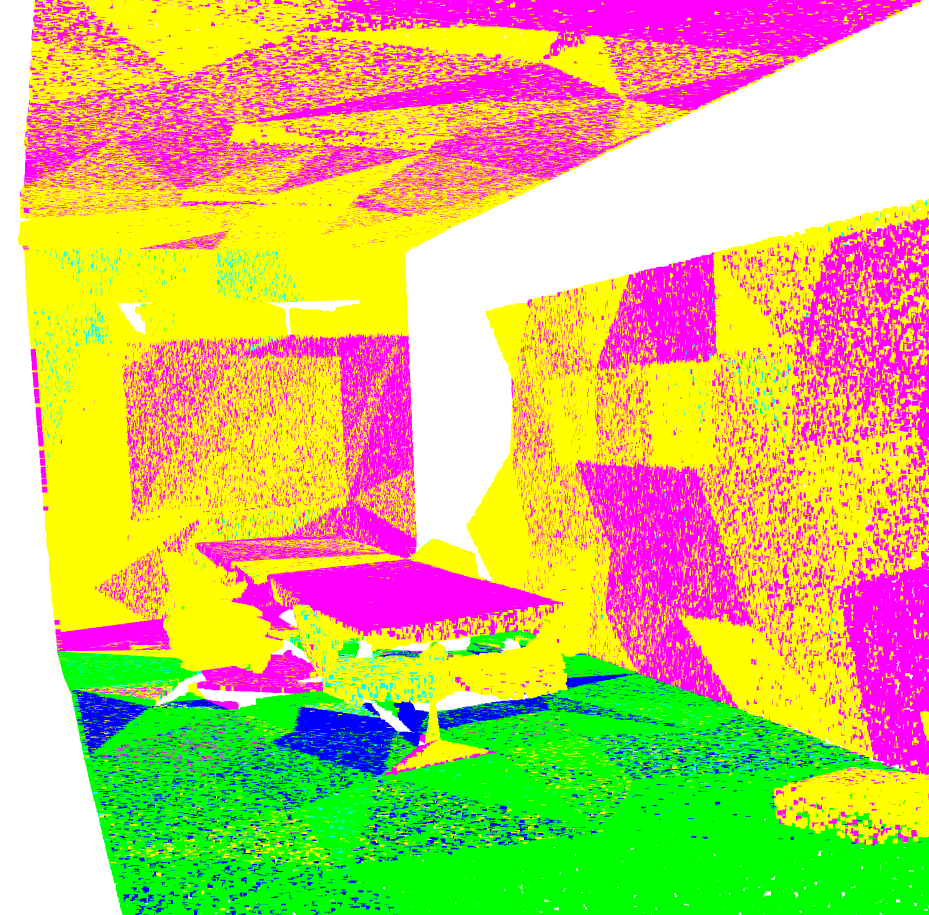
\includegraphics[width=0.33\textwidth, height=0.18\textheight]{images/seg_output/s3dis_DE/ocroom_1.png} \\
            
            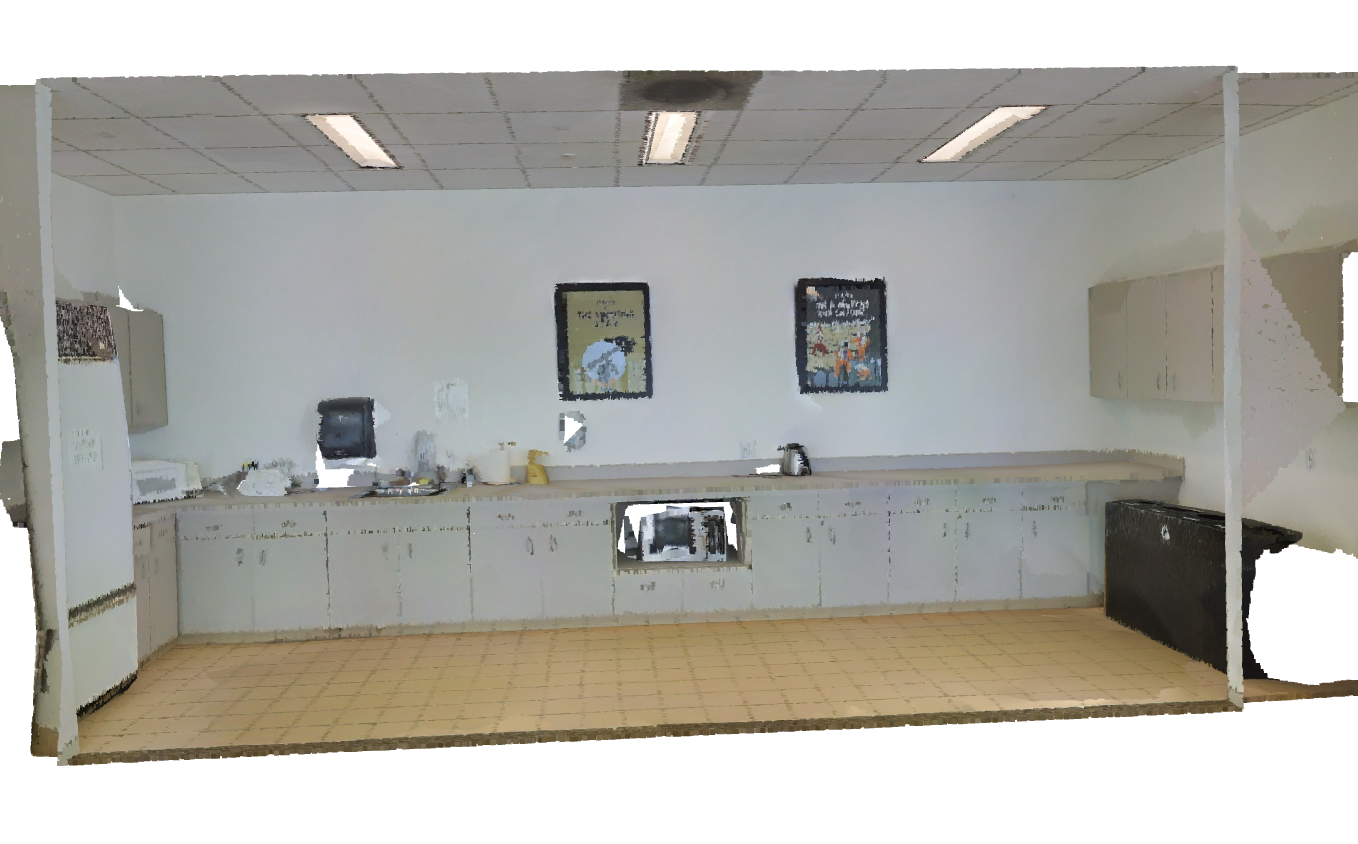
\includegraphics[width=0.33\textwidth, height=0.18\textheight]{images/seg_output/s3dis_DE/S3DIS_3_RGB.png} &
            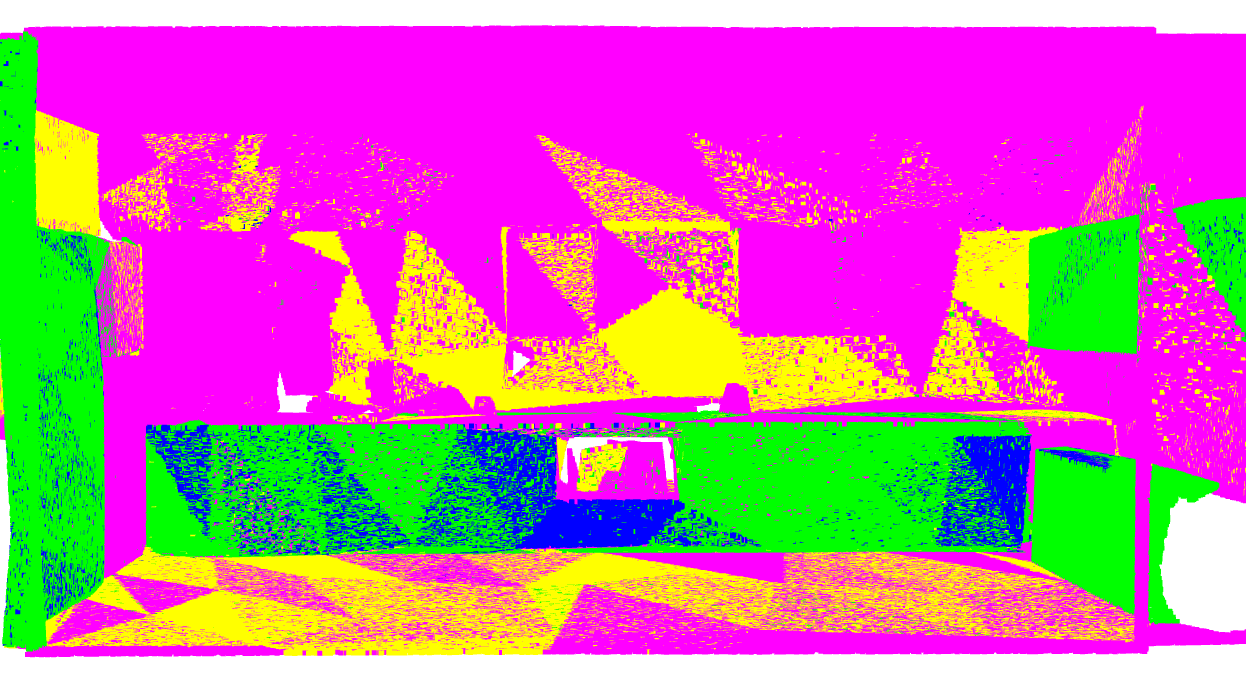
\includegraphics[width=0.33\textwidth, height=0.18\textheight]{images/seg_output/s3dis_DE/S3DIS_3_Pred.png}&
            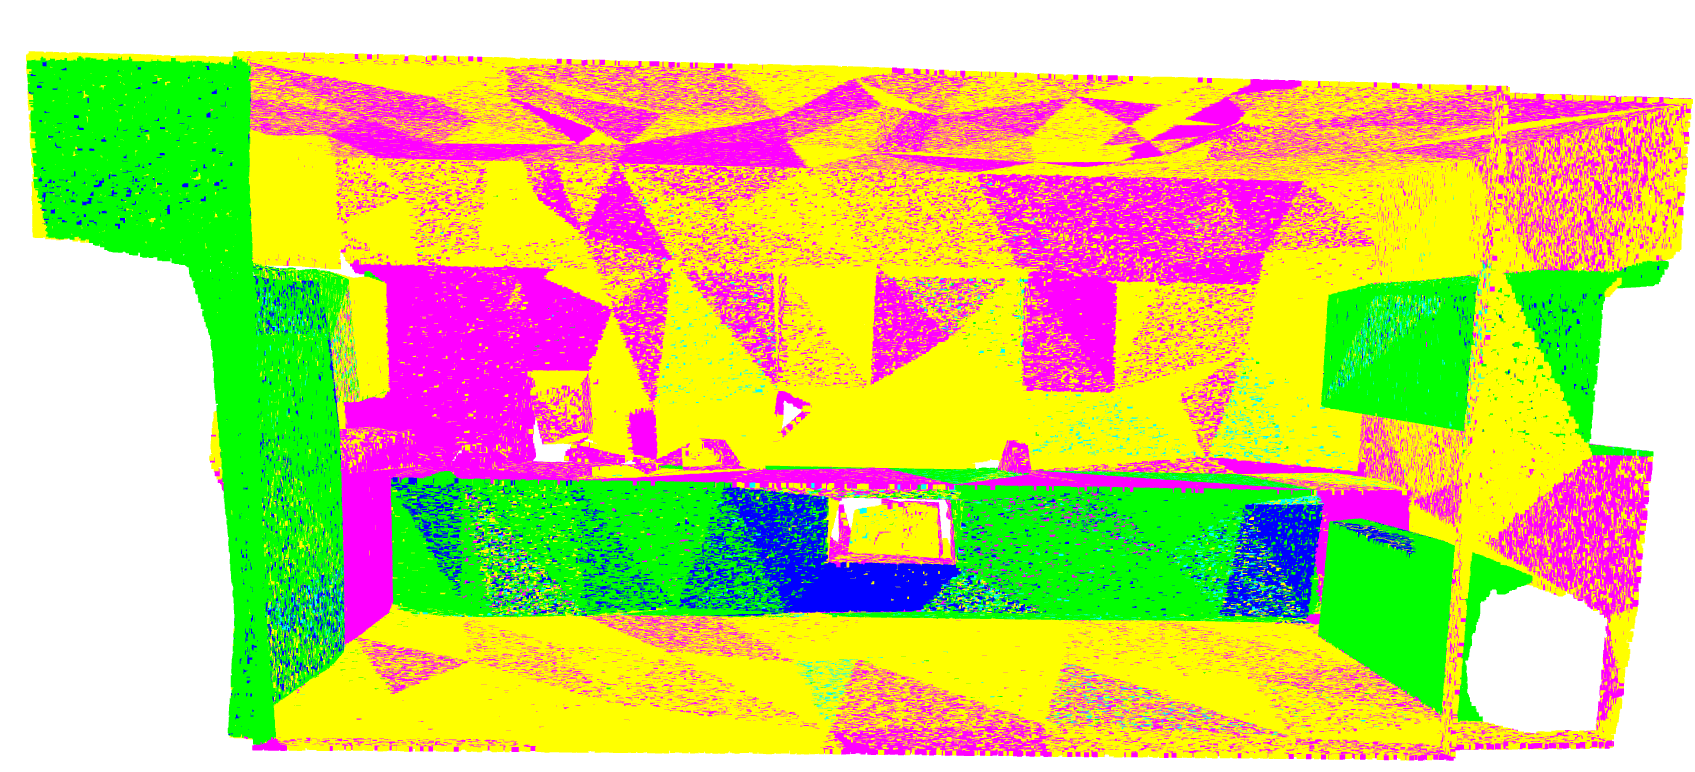
\includegraphics[width=0.33\textwidth, height=0.18\textheight]{images/seg_output/s3dis_DE/opantry_1.png} \\

            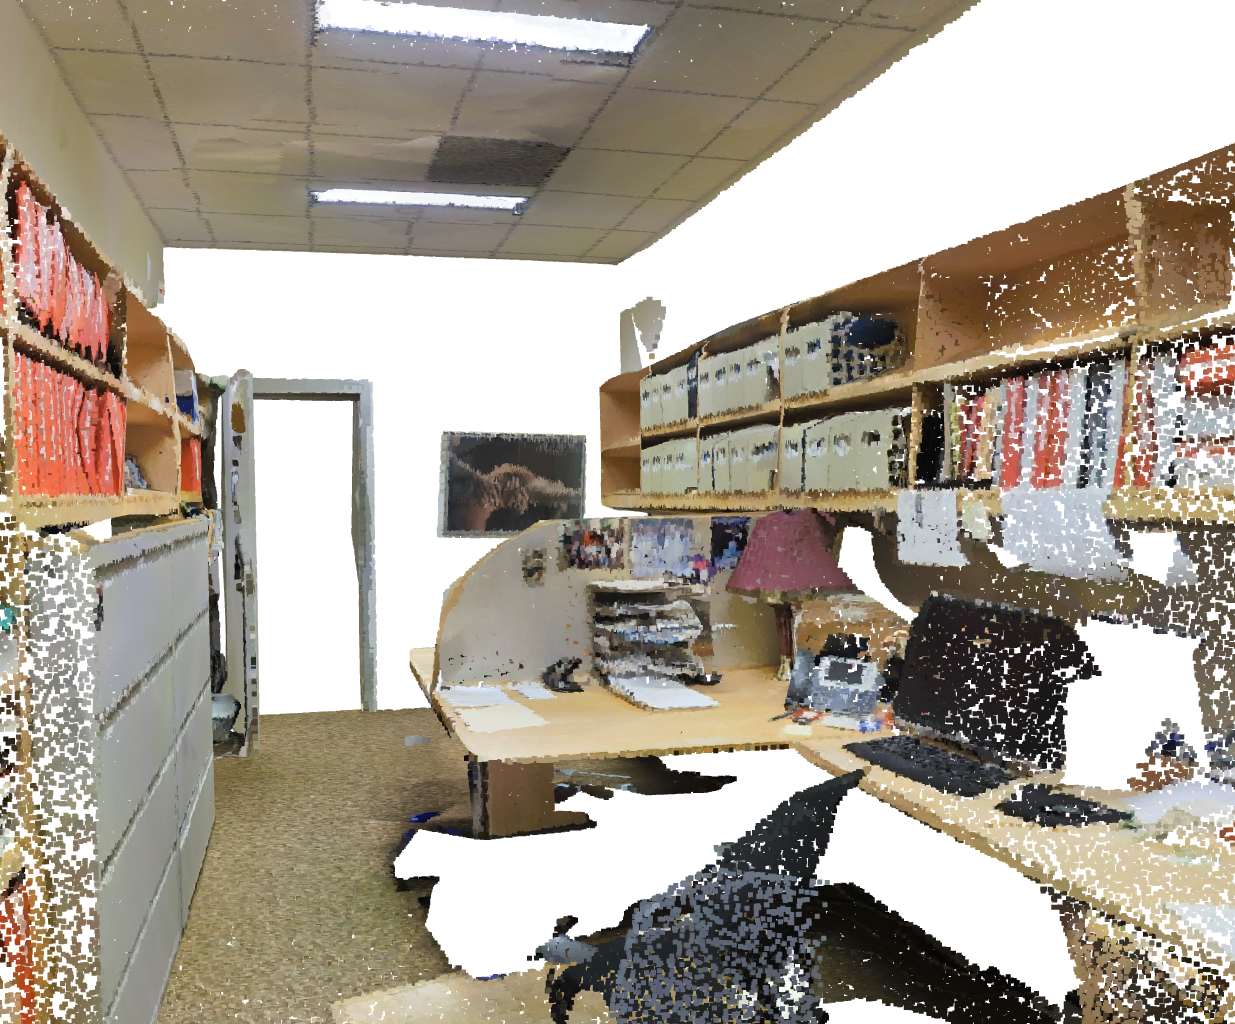
\includegraphics[width=0.33\textwidth, height=0.18\textheight]{images/seg_output/s3dis_DE/S3DIS_4_RGB.png} &
            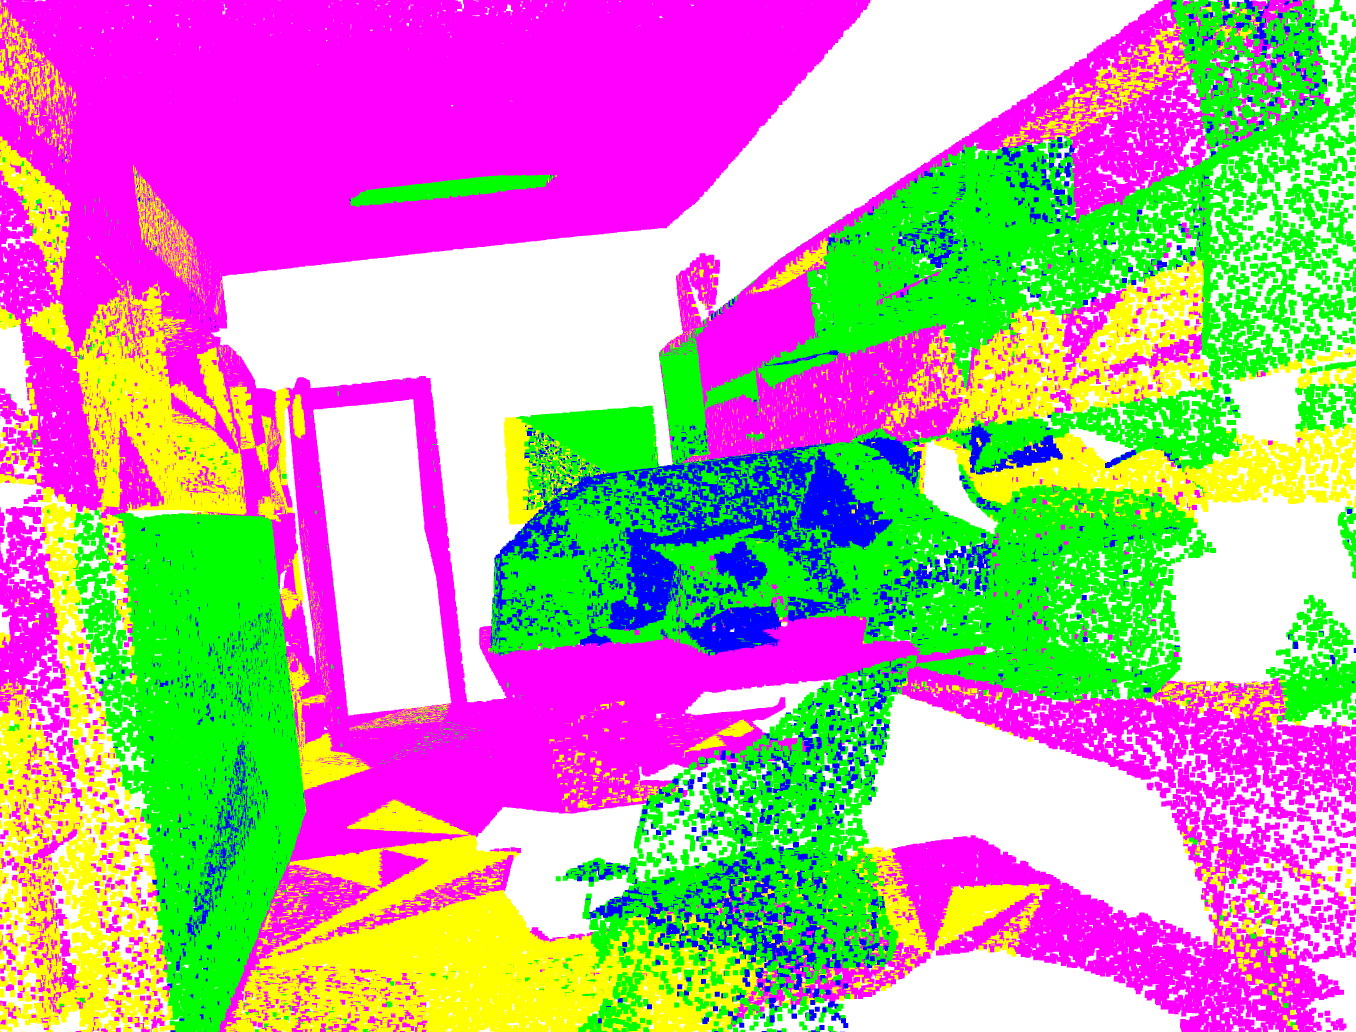
\includegraphics[width=0.33\textwidth, height=0.18\textheight]{images/seg_output/s3dis_DE/S3DIS_4_Pred.png}&
            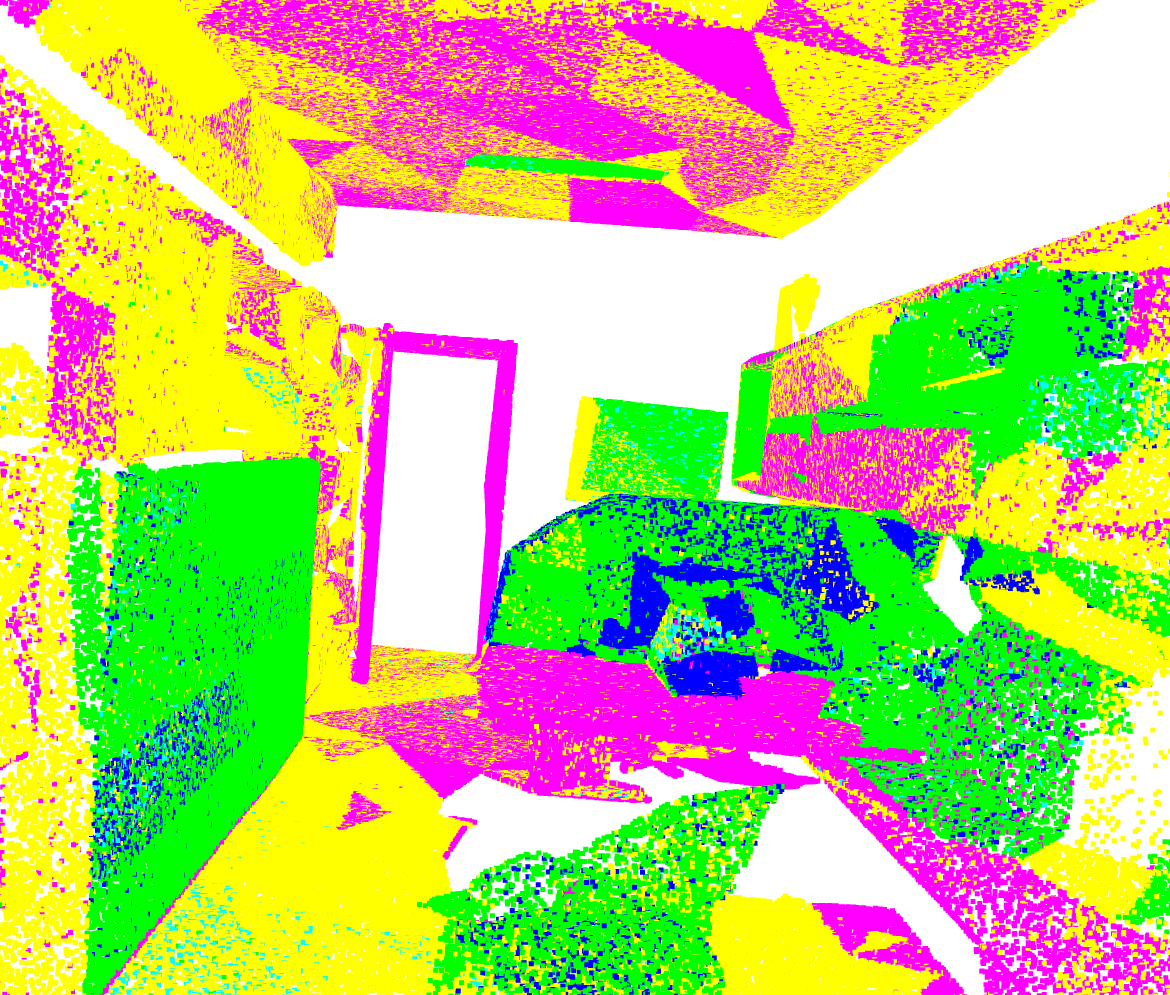
\includegraphics[width=0.33\textwidth, height=0.18\textheight]{images/seg_output/s3dis_DE/office_42.png} \\
        \end{tabular}
        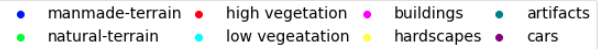
\includegraphics[scale=0.65]{images/legend.png}
        \caption{Output predictions of the RandLA-Net over the S3DIS dataset.}
        \label{fig:de_s3dis_vis}
    \end{figure*}
    %%%%%% Maximum probability (Semantic3D vs S3DIS) %%%%%%
    \subsection{Maximum Softmax Probability (MSP)}
    \label{sec:prob_sem3dvs3dis}
    In this experiment, we study the probability values of the ID dataset (Semantic3D), and OOD dataset (S3DIS) computed using Deep Ensembles and Flipout methods of RandLA-Net.
    We compute the average of the maximum softmax probability of all the points in the dataset, and this averaged value is called here the mean probability value.
    Figure~\ref{fig:msp_ensembles} and Figure~\ref{fig:msp_flipout} depicts the mean probability values across the ID (green) and OOD (red) datasets and their variance represented as error bars.
    Figure~\ref{fig:msp_ensembles} represents the change in mean probability value to ensemble size.
    Figure~\ref{fig:msp_flipout} represents the change in mean probability value to the number of passes in Flipout.
    Here, we represent the mean probability values across the odd number of ensembles size and the odd number of passes in case of flipout.
    \begin{figure}[h!]
        \centering
        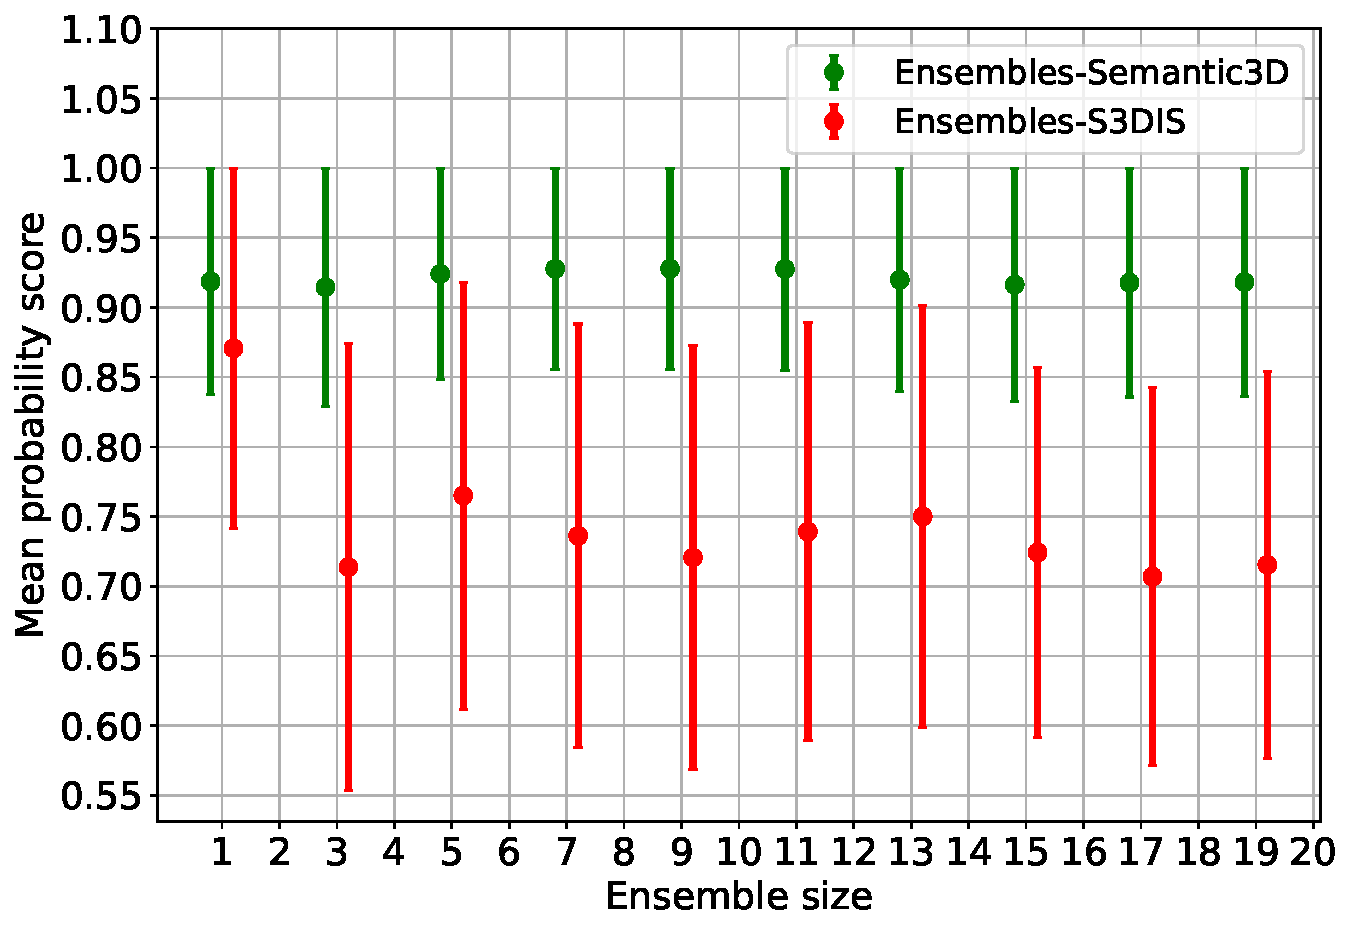
\includegraphics[scale=0.6]{images/MSP/Ensembles_MSP_cnc.pdf}
        \caption{MSP deep ensembles}
        \label{fig:msp_ensembles}
    \end{figure}

    \begin{figure}[h!]
        \centering
        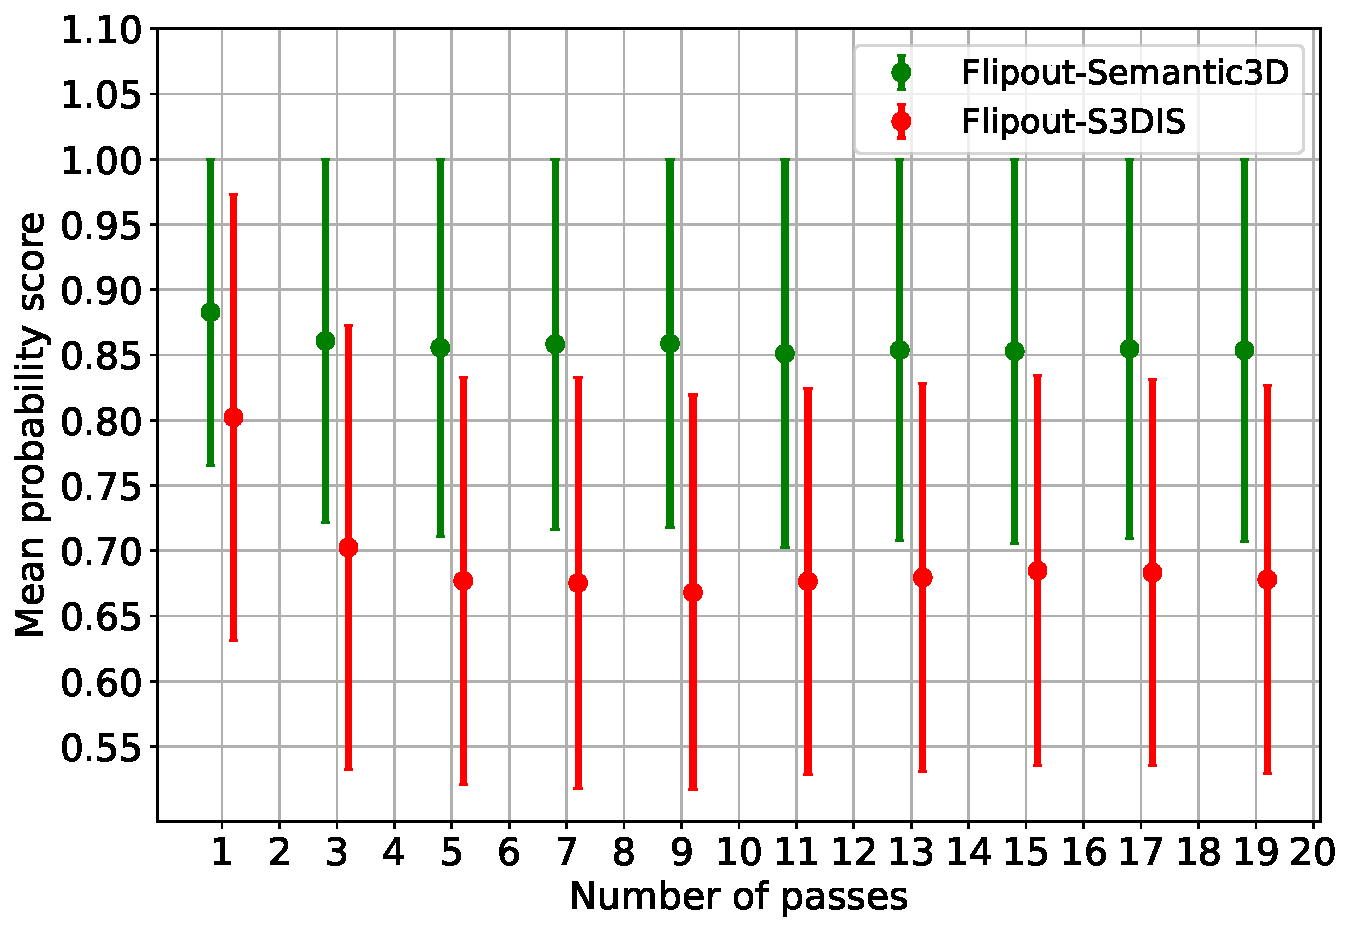
\includegraphics[scale=0.6]{images/MSP/Flipout_MSP_cnc.pdf}
        \caption{MSP flipout}
        \label{fig:msp_flipout}
    \end{figure}

    From Figure~\ref{fig:msp_ensembles}, we can infer that as the increase in ensemble size, the mean probability of the ID (Semantic3D) dataset remains stable.
    The variance is reduced until the ensemble size of 9 and then stabilizes.
    In the case of the OOD (S3DIS) dataset, we observe a decrement in mean probability value and then remain the same after an ensemble size of 3 with a larger variance.
    With the increase in ensemble size, we also observe that the overlap in the variance of ID and OOD is getting lower.
    This smaller overlap in higher ensemble size should result in higher OOD detection performance.
    In the case of Flipout, as in Figure~\ref{fig:msp_flipout} the mean probability and variance remain mostly the same for the ID dataset.
    With the OOD dataset, we observed a reduction in the mean probability value in the case of multiple passes.
    The variance from the Flipout is higher than the Deep Ensembles for the ID dataset.
    This phenomenon is to be expected because the Deep Ensembles combine predictions from various radomly initializated models and in the case of Flipout same model is used for multiple forward passes.
    % \textbf{Aim: } In this experiment, we study how the probability scores are distributed in Semantic3D and S3DIS datasets which are ID and OOD datasets respectively.
    % \begin{figure}[h!]
    %     \centering
    % %\begin{subfigure}{0.54\textwidth}
    % %        \includestandalone[scale=0.9]{images/mean_prob_sem3dvs3dis}
    %     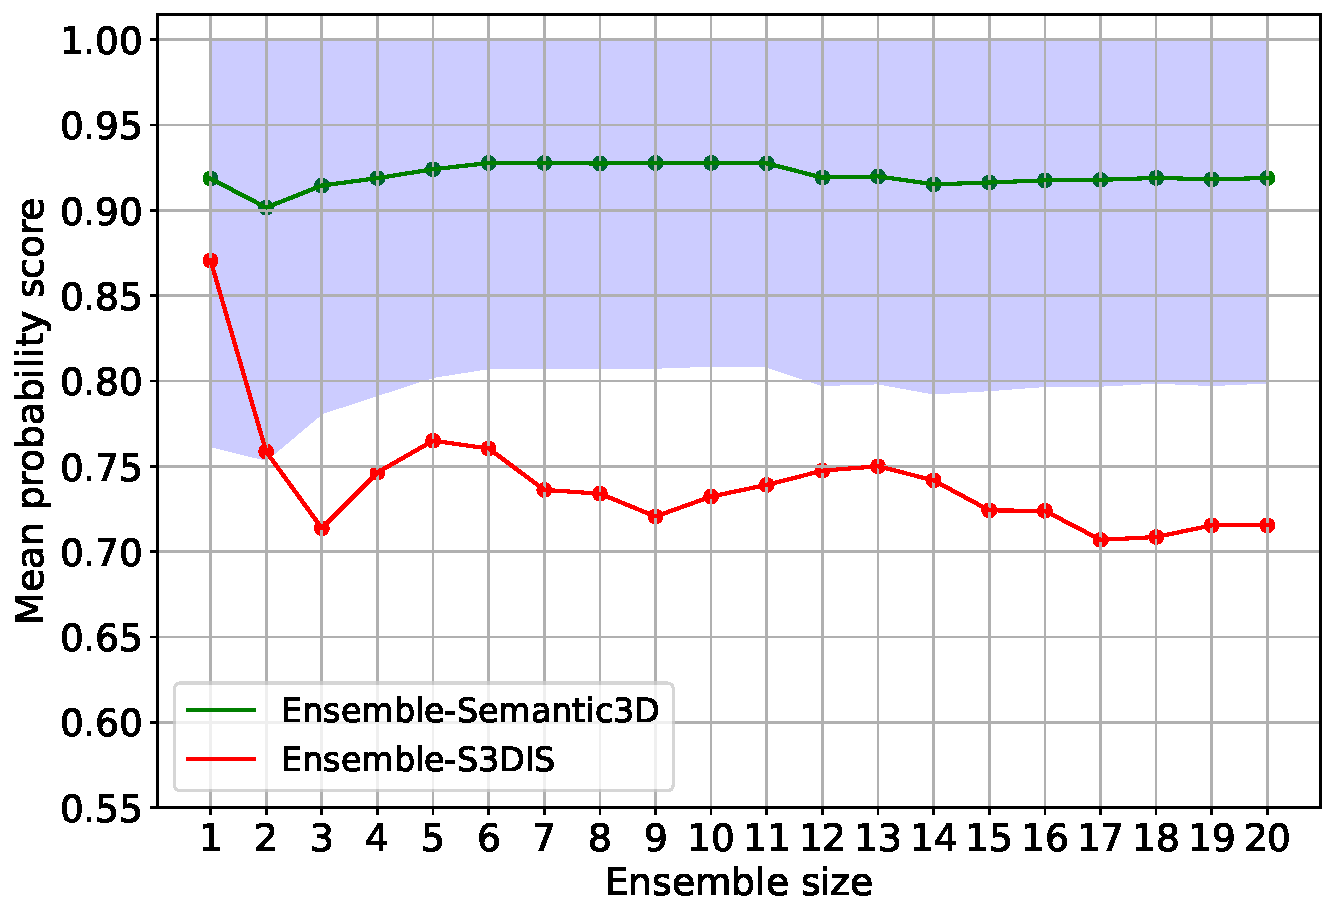
\includegraphics[scale=0.55]{images/Ensemble_MSP.pdf}
    %     \caption{}
    %     \label{fig:prob_sem3dvs3dis_de}    
    % %\end{subfigure}
    % \end{figure}
    % \begin{figure}[h!]
    %     \centering
    % %\begin{subfigure}{0.45\textwidth}
    % %       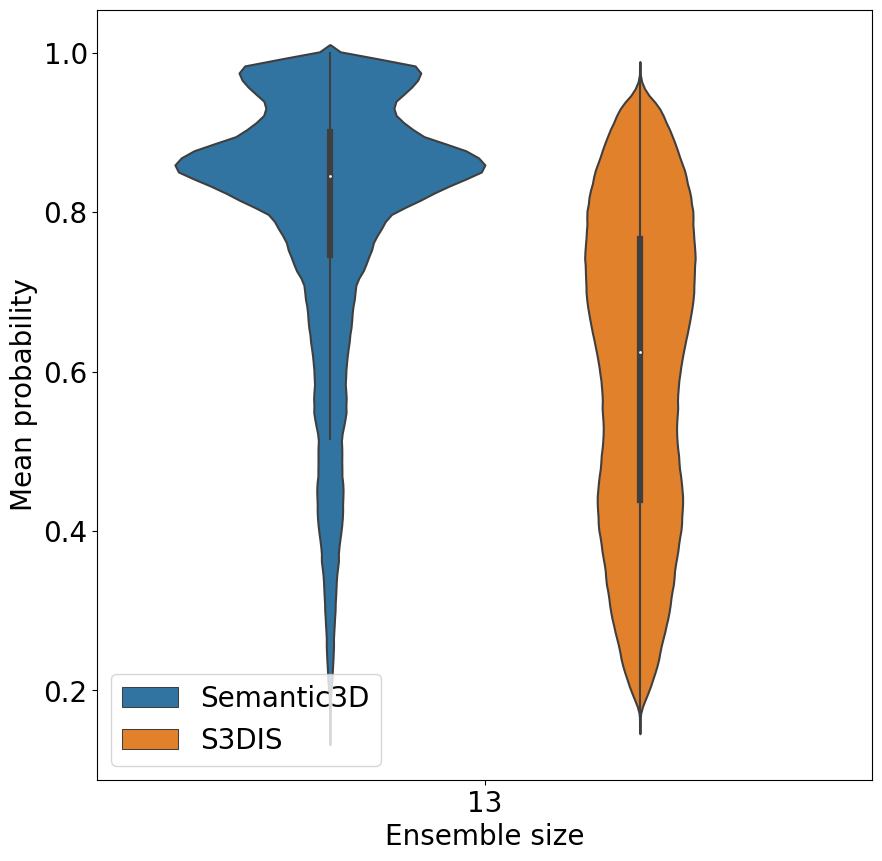
\includegraphics[scale=0.33]{images/violin_in_Max_predicted_probability.png}
    %     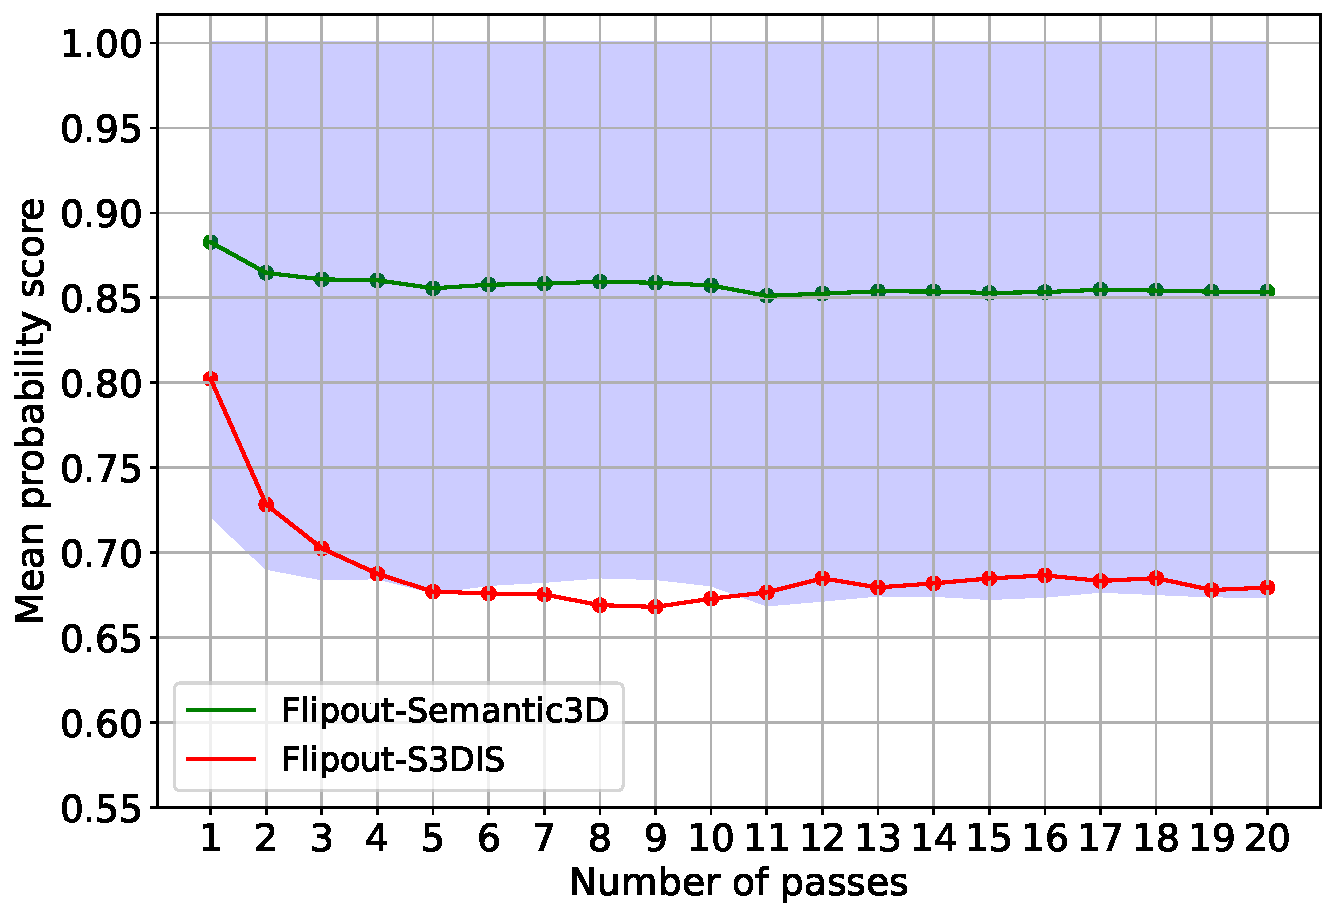
\includegraphics[scale=0.55]{images/Flipout_MSP.pdf}
    %     \caption{}
    %     \label{fig:13_sem3dvs3dis}
    % %\end{subfigure}
    % \end{figure}

    % \begin{figure}[h!]
    %     \centering
    %     \begin{subfigure}{0.98\textwidth}
    %         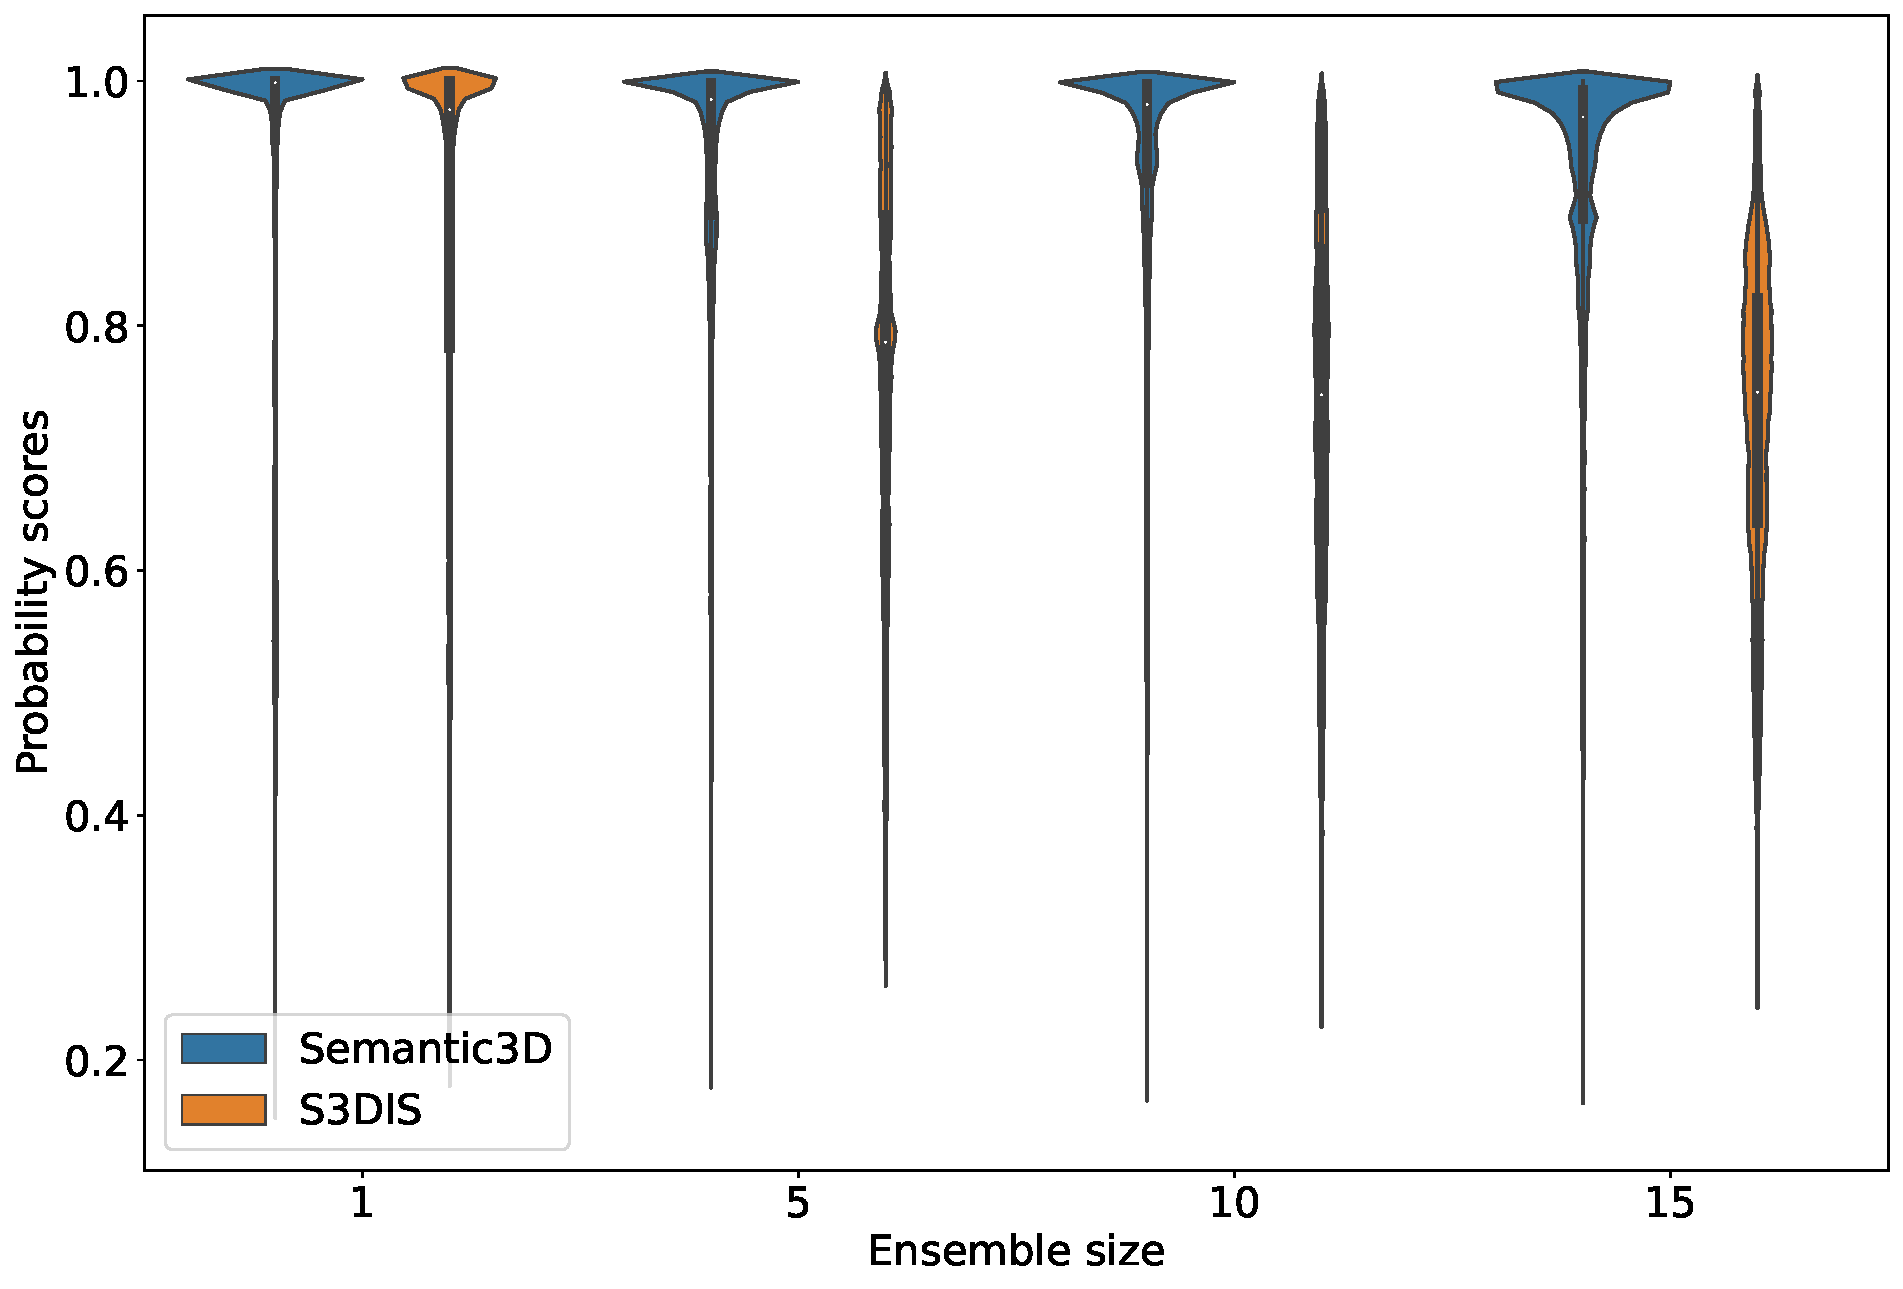
\includegraphics[width=0.98\textwidth, height=0.48\textheight]{images/violin_in_Probability_DE_plot.pdf}
    %     \end{subfigure}
    %     \begin{subfigure}{0.98\textwidth}
    %         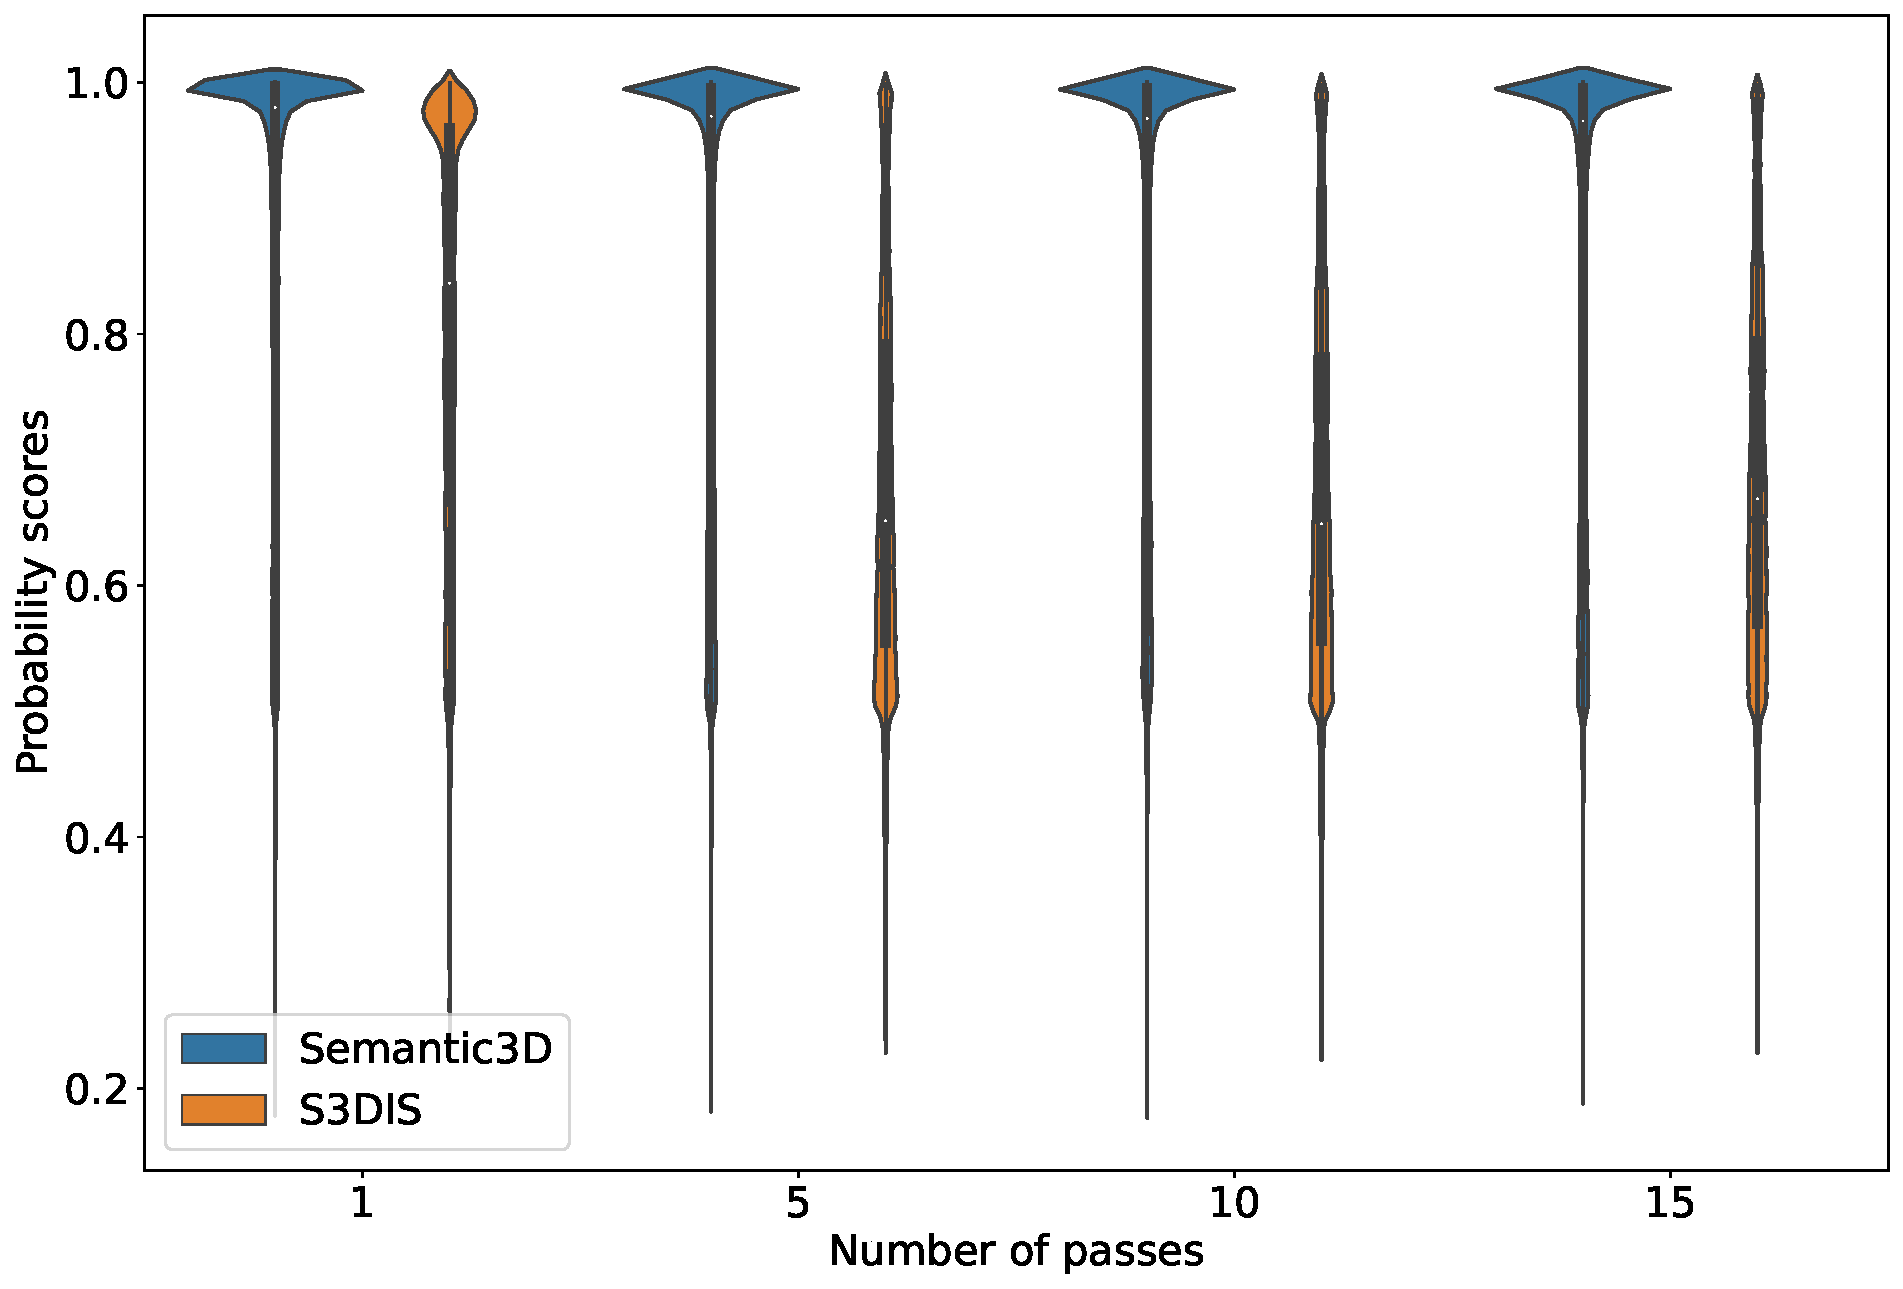
\includegraphics[width=0.98\textwidth, height=0.48\textheight]{images/violin_in_Probability_FOUT_plot.pdf}
    %     \end{subfigure}
    % \end{figure}
    % \begin{figure*}[h!]
    %     \centering
    %     \begin{tabular}{ccc}
    %         Ground Truth & Prediction & Probaility score \\
    %         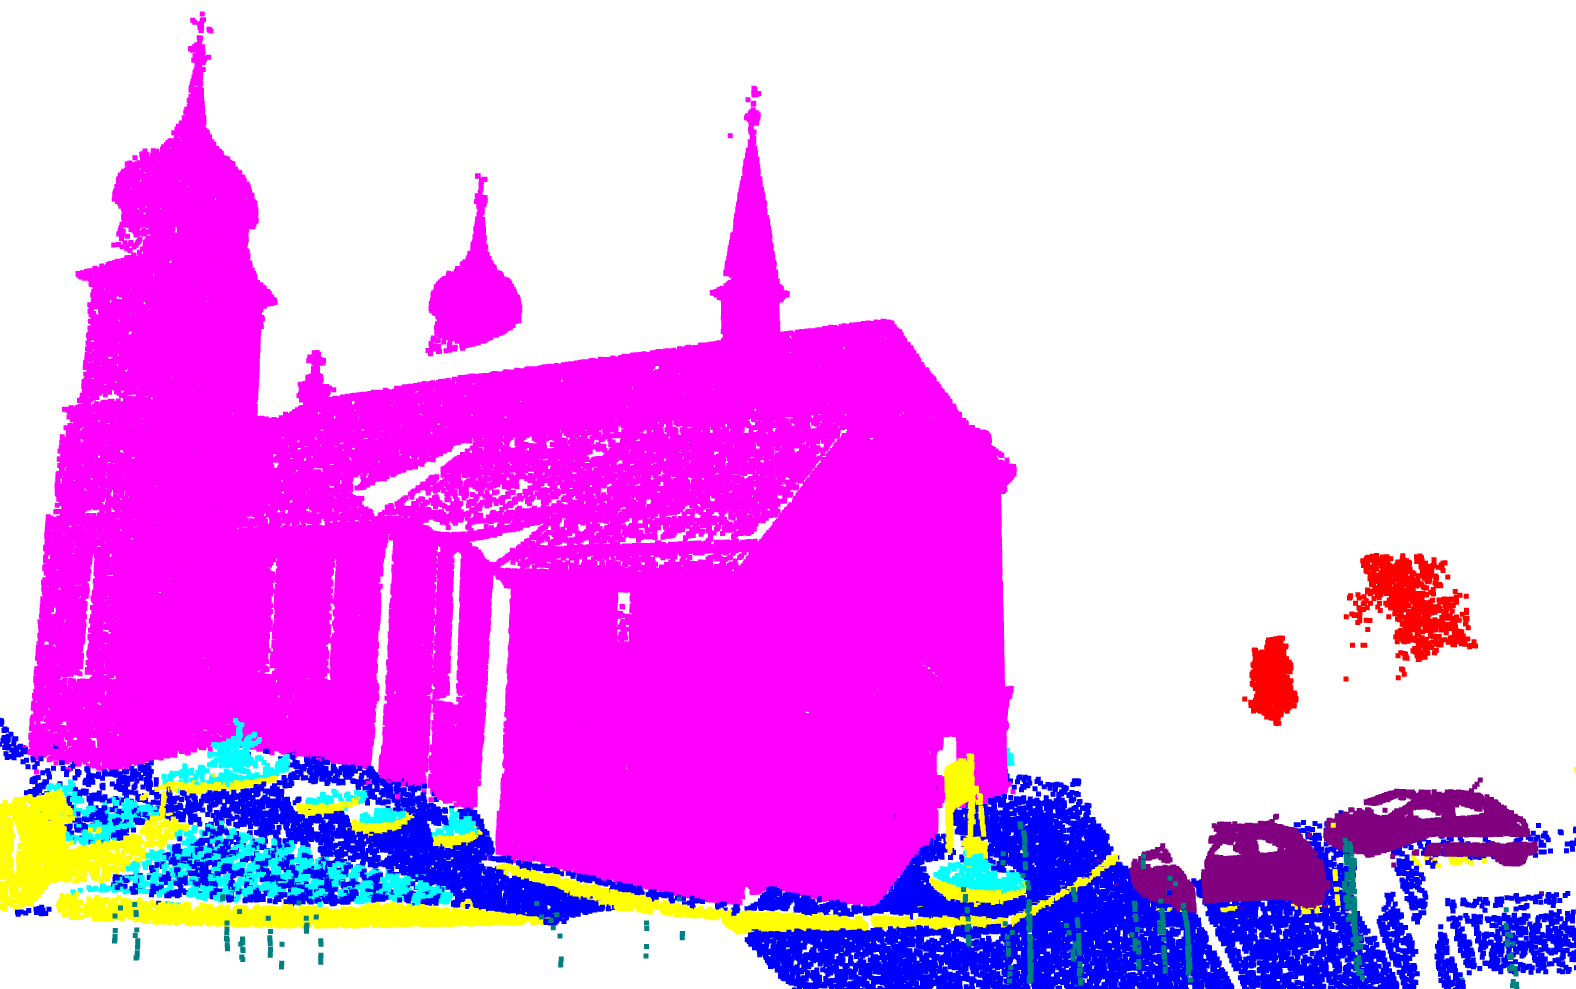
\includegraphics[width=0.33\textwidth, height=0.18\textheight]{images/seg_output/sem3d_seg_output/1_GT.png} &
    %         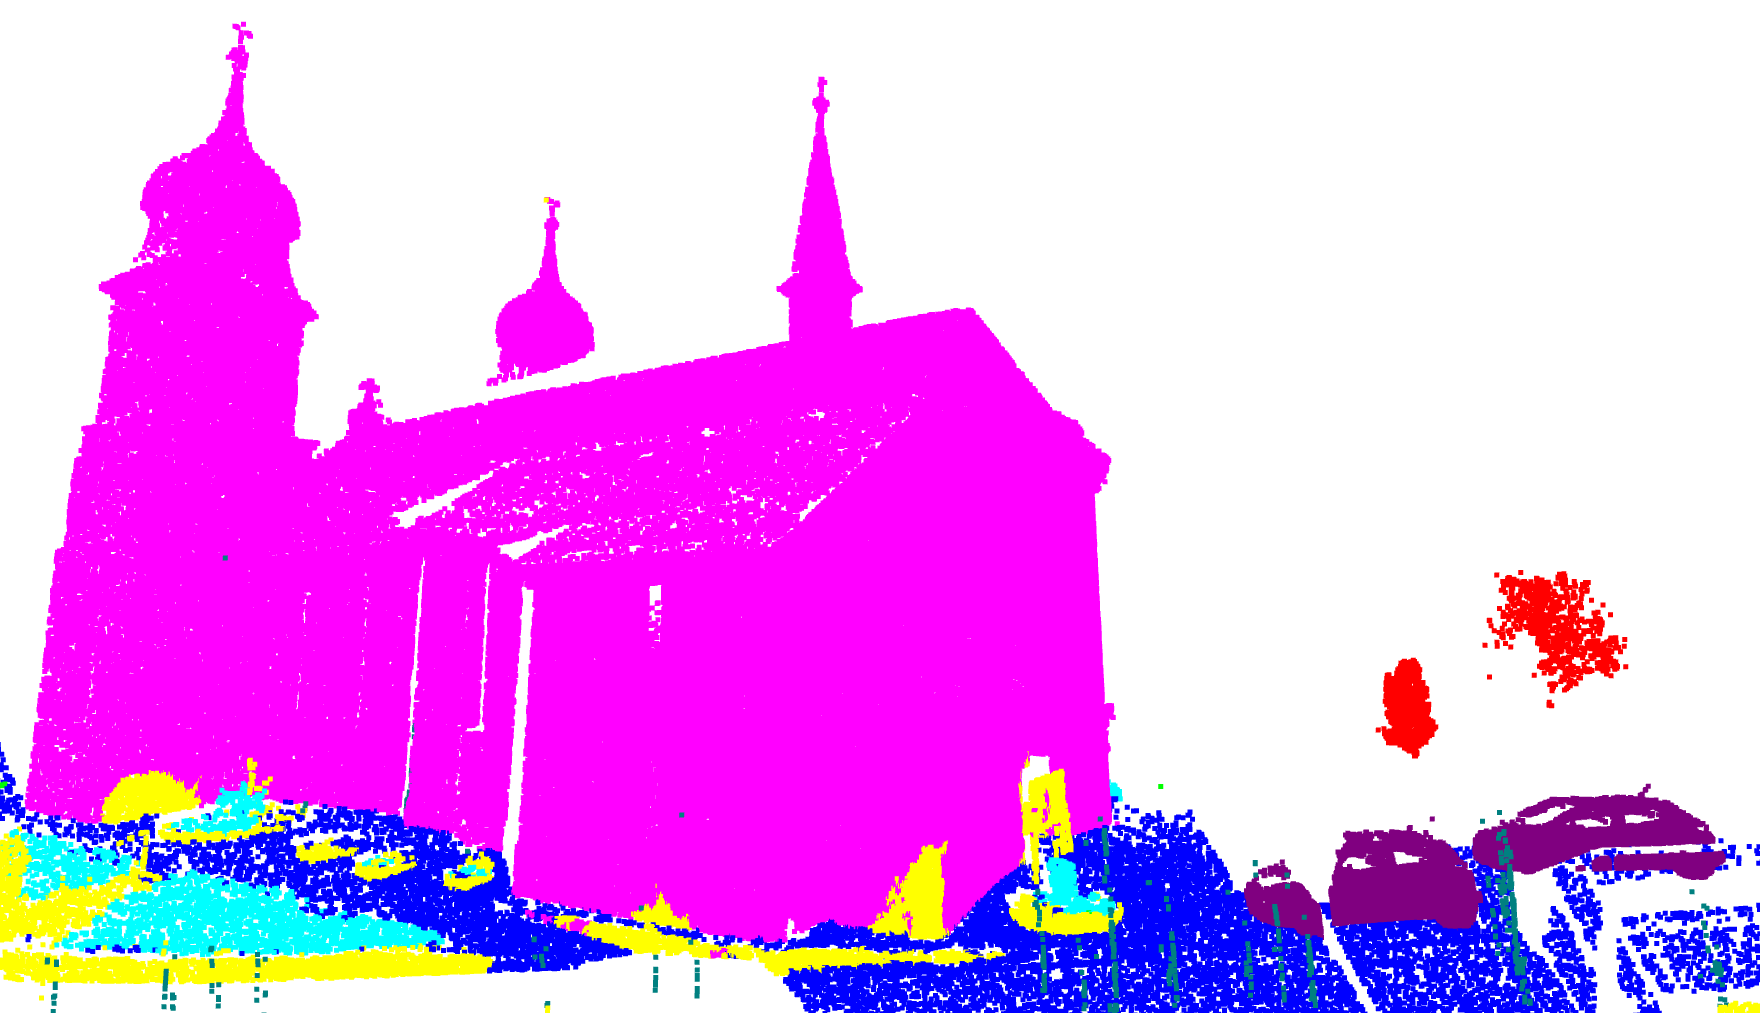
\includegraphics[width=0.33\textwidth, height=0.18\textheight]{images/seg_output/sem3d_seg_output/1_Pred.png}& 
    %         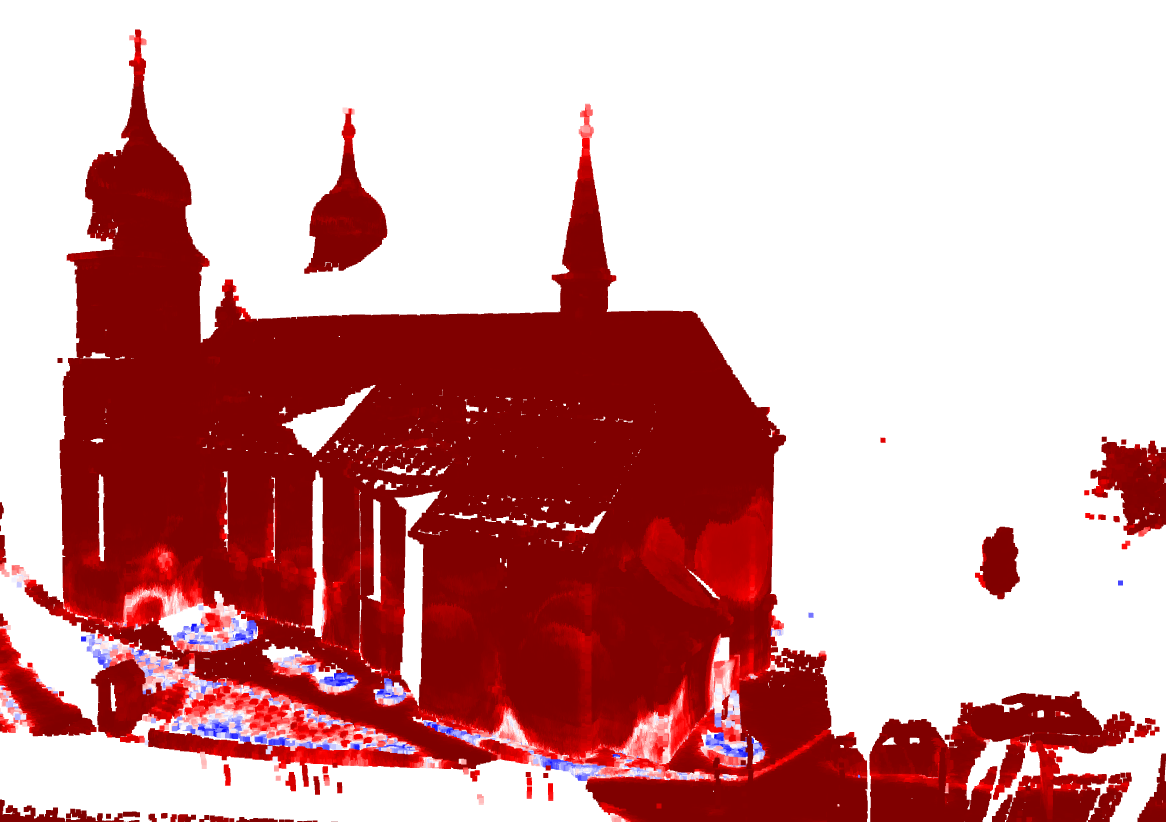
\includegraphics[width=0.33\textwidth, height=0.18\textheight]{images/seg_output/sem3d_seg_output/1_max_prob.png}\\

    %         \includegraphics[width=0.33\textwidth, height=0.18\textheight]{images/seg_output/sem3d_seg_output/2_GT.png} &
    %         \includegraphics[width=0.33\textwidth, height=0.18\textheight]{images/seg_output/sem3d_seg_output/2_Pred.png}& 
    %         \includegraphics[width=0.33\textwidth, height=0.18\textheight]{images/seg_output/sem3d_seg_output/2_max_prob.png}\\

    %         \includegraphics[width=0.33\textwidth, height=0.18\textheight]{images/seg_output/sem3d_seg_output/3_GT.png} &
    %         \includegraphics[width=0.33\textwidth, height=0.18\textheight]{images/seg_output/sem3d_seg_output/3_Pred.png}& 
    %         \includegraphics[width=0.33\textwidth, height=0.18\textheight]{images/seg_output/sem3d_seg_output/3_max_prob.png}\\
    %     \end{tabular}
    %     \includegraphics[scale=0.213]{images/color_legend.pdf}
    %     \includegraphics[scale=0.65]{images/legend.png}
    %     \caption{Perpoint probability visualization of the semantic3D dataset.}
    % \end{figure*}

    % \begin{figure*}[h!]
    %     \centering
    %     \begin{tabular}{cc}
    %         Prediction & Probaility score \\
    %         \includegraphics[width=0.33\textwidth, height=0.18\textheight]{images/seg_output/s3dis_DE/S3DIS_1_Pred.png}& 
    %         \includegraphics[width=0.33\textwidth, height=0.18\textheight]{images/seg_output/s3dis_DE/S3DIS_1_prob.png}\\

    %         \includegraphics[width=0.33\textwidth, height=0.18\textheight]{images/seg_output/s3dis_DE/S3DIS_2_Pred.png}& 
    %         \includegraphics[width=0.33\textwidth, height=0.18\textheight]{images/seg_output/s3dis_DE/S3DIS_2_prob.png}\\

    %         \includegraphics[width=0.33\textwidth, height=0.18\textheight]{images/seg_output/s3dis_DE/S3DIS_3_Pred.png}& 
    %         \includegraphics[width=0.33\textwidth, height=0.18\textheight]{images/seg_output/s3dis_DE/S3DIS_3_prob.png}\\

    %         \includegraphics[width=0.33\textwidth, height=0.18\textheight]{images/seg_output/s3dis_DE/S3DIS_4_Pred.png}& 
    %         \includegraphics[width=0.33\textwidth, height=0.18\textheight]{images/seg_output/s3dis_DE/S3DIS_4_prob.png}\\
    %     \end{tabular}
    %     \includegraphics[scale=0.213]{images/color_legend.pdf}
    %     \includegraphics[scale=0.65]{images/legend.png}
    %     \caption{Perpoint probability visualization of the S3DIS dataset.}
    % \end{figure*}

    % \begin{figure}[h!]
    %     \begin{subfigure}{0.495\textwidth}
    %         \includegraphics[scale=0.35]{images/ensemble_probability_sem3dvs3dis_AUROC.pdf}
    %     \end{subfigure}
    %     \begin{subfigure}{0.495\textwidth}
    %         \includegraphics[scale=0.35]{images/flipout_probability_sem3dvs3dis_AUROC.pdf}
    %     \end{subfigure}
    %     \begin{subfigure}{0.98\textwidth}
    %         \centering
    %         \includegraphics[scale=0.35]{images/dropout_probability_sem3dvs3dis_AUROC.pdf}
    %     \end{subfigure}
    %     \caption{Ensmeble Vs Flipout Vs Dropout- Probability scores}
    % \end{figure}
    %%%%%% Entropy (Semantic3D vs S3DIS) %%%%%%
    \subsection{Entropy}
    \label{sec:ent_sem3dvs3dis}
    % \begin{figure}[h!]
    %     \centering
    % %\begin{subfigure}{0.54\textwidth}
    % %        \includestandalone[scale=0.9]{images/mean_prob_sem3dvs3dis}
    %     \includegraphics[scale=0.55]{images/Ensemble_Entropy.pdf}
    %     \caption{}
    %     \label{fig:ent_sem3dvs3dis_de}    
    % %\end{subfigure}
    % \end{figure}
    % \begin{figure}[h!]
    %     \centering
    % %\begin{subfigure}{0.45\textwidth}
    % %       \includegraphics[scale=0.33]{images/violin_in_Max_predicted_probability.png}
    %     \includegraphics[scale=0.55]{images/Flipout_Entropy.pdf}
    %     \caption{}
    %     \label{fig:ent_sem3dvs3dis_fout}
    % %\end{subfigure}
    % \end{figure}
    % \begin{figure}[h!]
    %     \centering
    %     \begin{subfigure}{0.98\textwidth}
    %         \includegraphics[width=0.98\textwidth, height=0.48\textheight]{images/violin_in_Entropy_DE_plot.pdf}
    %     \end{subfigure}
    %     \begin{subfigure}{0.98\textwidth}
    %         \includegraphics[width=0.98\textwidth, height=0.48\textheight]{images/violin_in_Entropy_FOUT_plot.pdf}
    %     \end{subfigure}
    % \end{figure}
    % \begin{figure*}[h!]
    %     \begin{tabular}{ccc}
    %         Ground Truth & Prediction & Entropy score \\
    %         \includegraphics[width=0.33\textwidth, height=0.18\textheight]{images/seg_output/sem3d_seg_output/1_GT.png} &
    %         \includegraphics[width=0.33\textwidth, height=0.18\textheight]{images/seg_output/sem3d_seg_output/1_Pred.png}& 
    %         \includegraphics[width=0.33\textwidth, height=0.18\textheight]{images/seg_output/sem3d_seg_output/1_Entropy.png}\\

    %         \includegraphics[width=0.33\textwidth, height=0.18\textheight]{images/seg_output/sem3d_seg_output/2_GT.png} &
    %         \includegraphics[width=0.33\textwidth, height=0.18\textheight]{images/seg_output/sem3d_seg_output/2_Pred.png}& 
    %         \includegraphics[width=0.33\textwidth, height=0.18\textheight]{images/seg_output/sem3d_seg_output/2_Entropy.png}\\

    %         \includegraphics[width=0.33\textwidth, height=0.18\textheight]{images/seg_output/sem3d_seg_output/3_GT.png} &
    %         \includegraphics[width=0.33\textwidth, height=0.18\textheight]{images/seg_output/sem3d_seg_output/3_Pred.png}& 
    %         \includegraphics[width=0.33\textwidth, height=0.18\textheight]{images/seg_output/sem3d_seg_output/3_Entropy.png}\\
    %     \end{tabular}
    %     \includegraphics[scale=0.213]{images/color_legend.pdf}
    %     \includegraphics[scale=0.65]{images/legend.png}
    %     \caption{Perpoint entropy visualization of the semantic3D dataset.}
    % \end{figure*}

    % \begin{figure*}[h!]
    %     \centering
    %     \begin{tabular}{cc}
    %         Prediction & Entropy score \\
    %         \includegraphics[width=0.33\textwidth, height=0.18\textheight]{images/seg_output/s3dis_DE/S3DIS_1_Pred.png}& 
    %         \includegraphics[width=0.33\textwidth, height=0.18\textheight]{images/seg_output/s3dis_DE/S3DIS_1_Entropy.png}\\

    %         \includegraphics[width=0.33\textwidth, height=0.18\textheight]{images/seg_output/s3dis_DE/S3DIS_2_Pred.png}& 
    %         \includegraphics[width=0.33\textwidth, height=0.18\textheight]{images/seg_output/s3dis_DE/S3DIS_2_Entropy.png}\\

    %         \includegraphics[width=0.33\textwidth, height=0.18\textheight]{images/seg_output/s3dis_DE/S3DIS_3_Pred.png}& 
    %         \includegraphics[width=0.33\textwidth, height=0.18\textheight]{images/seg_output/s3dis_DE/S3DIS_3_Entropy.png}\\

    %         \includegraphics[width=0.33\textwidth, height=0.18\textheight]{images/seg_output/s3dis_DE/S3DIS_4_Pred.png}& 
    %         \includegraphics[width=0.33\textwidth, height=0.18\textheight]{images/seg_output/s3dis_DE/S3DIS_4_Entropy.png}\\
    %     \end{tabular}
    %     \includegraphics[scale=0.213]{images/color_legend.pdf}
    %     \includegraphics[scale=0.65]{images/legend.png}
    %     \caption{Perpoint entropy visualization of the S3DIS dataset.}
    % \end{figure*}
    % \begin{figure}[h!]
    %     \begin{subfigure}{0.495\textwidth}
    %         \includegraphics[scale=0.35]{images/ensemble_entropy_sem3dvs3dis_AUROC.pdf}
    %     \end{subfigure}
    %     \begin{subfigure}{0.495\textwidth}
    %         \includegraphics[scale=0.35]{images/flipout_entropy_sem3dvs3dis_AUROC.pdf}
    %     \end{subfigure}
    %     \begin{subfigure}{0.98\textwidth}
    %         \centering
    %         \includegraphics[scale=0.35]{images/dropout_probability_sem3dvs3dis_AUROC.pdf}
    %     \end{subfigure}
    %     \caption{Ensemble Vs Flipout Vs Dropout- Entropy scores}
    % \end{figure}



    \section{OOD Benchmark - Semantic3D vs Semantic3D without color}
    \subsection{Deep ensembles}
    % \begin{table}[h!]
    %     \resizebox{\textwidth}{!}{%
    %     \begin{tabular}{c|c|cccccccc|c}
    %     %\textbf{\#Ensembles} & \textbf{MeanIOU} & \textbf{Accuracy} & \textbf{Manmadeterrain} & \textbf{Naturalterrain} & \textbf{Highvegetation} & \textbf{Lowvegetation} & \textbf{Buildings} & \textbf{Hardscapes} & \textbf{Scanningartifacts} & \textbf{Cars} \\ \hline
    %     & & \multicolumn{7}{c}{\textbf{IoU per class}} & \\ \hline
    %     \textbf{\#Ensembles} & \textbf{MeanIOU} & \textbf{C1} & \textbf{C2} & \textbf{C3} & \textbf{C4} & \textbf{C5} & \textbf{C6} & \textbf{C7} & \textbf{C8} & \textbf{Accuracy} \\ \hline
    %     1& 68.19& 94.55& 81.19& 84.67& 29.43& 81.37& 18.85& 64.74& 90.74& 88.78 \\
    %     5& 69.51& 94.73& 81.92& 84.42& 28.05& \textbf{86.41}& 28.50& 61.03& 91.03& 90.04 \\
    %     10& 69.97& 95.25& 83.73& 86.63& 30.36& 84.13& 18.60& \textbf{66.01}& 92.61& 89.94 \\
    %     15& 70.32& 95.27& 83.54& \textbf{88.22}& \textbf{32.19}& 84.82& 26.17& 61.67& 90.75& \textbf{90.57} \\
    %     20& \textbf{70.80}& \textbf{95.55}& \textbf{84.11}& 86.65& 29.60& 85.41& \textbf{29.58}& 62.47& \textbf{93.06}& 90.56 \\
    %     \end{tabular}%
    %     }
    %     \caption{Illustration of performance of RandLA-Net on Semantic3D over number of ensembles. meanIOU and IOU per class and overall accuracy are represented here.
    %     C1 to C8 are the classes of Semantic3D which are Manmadeterrain, Naturalterrain, Highvegetation, Lowvegetation, Buildings, Hardscapes, Scanningartifacts, and Cars.}
    % \end{table}

    % \begin{table}[h!]
    %     \resizebox{\textwidth}{!}{%
    %     \begin{tabular}{c|c|cccccccc|c}
    %     %\textbf{\#Ensembles} & \textbf{MeanIOU} & \textbf{Accuracy} & \textbf{Manmadeterrain} & \textbf{Naturalterrain} & \textbf{Highvegetation} & \textbf{Lowvegetation} & \textbf{Buildings} & \textbf{Hardscapes} & \textbf{Scanningartifacts} & \textbf{Cars} \\ \hline
    %     & & \multicolumn{7}{c}{\textbf{IoU per class}} & \\ \hline
    %     \textbf{\#Ensembles} & \textbf{MeanIOU} & \textbf{C1} & \textbf{C2} & \textbf{C3} & \textbf{C4} & \textbf{C5} & \textbf{C6} & \textbf{C7} & \textbf{C8} & \textbf{Accuracy} \\ \hline
    %     1& 47.96&78.67&7.21&78.63&23.54&85.37&15.48&45.96&48.83&80.26\\
    %     5& 49.66&80.68&4.49&79.06&26.87&84.87&16.64&48.79&55.85&81.62\\
    %     10& 50.39&80.86&5.17&78.97&27.25&84.52&16.75&48.02&61.54&81.65\\
    %     15& 50.33&81.02&5.04&77.25&27.52&83.18&16.53&47.81&64.25&81.25\\
    %     20& 50.24&81.01&5.15&77.20&27.3&83.60&17.07&47.74&62.83&81.29\\
    %     \end{tabular}%
    %     }
    %     \caption{Illustration of performance of RandLA-Net on Semantic3D wihtout color over number of ensembles. meanIOU and IOU per class and overall accuracy are represented here.
    %     C1 to C8 are the classes of Semantic3D which are Manmadeterrain, Naturalterrain, Highvegetation, Lowvegetation, Buildings, Hardscapes, Scanningartifacts, and Cars.}
    % \end{table}

    \subsection{Flipout}

    \subsection{Maximum Softmax probability (MSP)}
    % \begin{figure}[h!]
    %     \centering
    %     \includegraphics[scale=0.55]{images/Ensemble_MSP_color_no_color.pdf}
    %     \caption{Ensemble Semantic3D vs Semantic3D no color - MSP}
    % \end{figure}
    % \begin{figure}
    %     \centering
    %     \includegraphics[scale=0.55]{images/Ensemble_probability_sem3dvsnocolorAUROC.pdf}
    % \end{figure}
    \subsection{Entropy}
    % \begin{figure}[h!]
    %     \centering\includegraphics[scale=0.55]{images/Ensemble_Entropy_color_no_color.pdf}
    %     \caption{Ensemble Semantic3D vs Semantic3D no color - Entropy}
    % \end{figure}
    % \begin{figure}
    %     \centering
    %     \includegraphics[scale=0.55]{images/Ensemble_entropy_sem3dvsnocolorAUROC.pdf}
    % \end{figure}

    \section{OOD detection evaluation}
\end{document}
